
\section{Previous Clock Deskew Implementation: Current-Starved Delay Stage}

The preceding implementation of the programmable delay stage used for clock deskewing was founded on a current-starved delay element. This architecture comprises eight distinct delay paths, each dedicated to the deskewing of one of eight clock signals, which are phase-shifted by 45 degrees relative to each other.


The delay stage of the previous implementation is controlled by modulating the gate voltage of the pull-up and pull-down transistors within current-starved inverters. This bias voltage is generated by an external \gls{dac} that limits the charging and discharging current at the inverter's output node. By adjusting this current, the rise and fall times of the output signal are controlled, thereby adjusting the delay. The full schematic of this architecture, including the diode-based \gls{dac} that individually biases the PMOS and NMOS branches for duty-cycle correction, is shown in Appendix~\ref{app:cs_delay_details} (Fig.~\ref{fig:current_starved_delay_stage} and Fig.~\ref{fig:current_starved_dac}).

A feature of this design is that the pull-up (PMOS) and pull-down (NMOS) branches of each current-starved inverter are individually addressable. This allows for independent control over the rising and falling signal edges, providing a mechanism for duty-cycle correction.

The control \gls{dac} for the current-starved inverters is implemented using diode-based \gls{dac}s. Structurally, each \gls{dac} resembles an inverter with an enable (EN) signal controlling an NMOS and PMOS pair. The path between the drains of the input transistors and the output is connected to a series of diodes whose number sets the strength of each branch. Multiple \gls{dac}s share a common output node whose voltage adjusts the current limits of the current-starved inverters, thereby tuning the delay.



A simple examination of this design highlighted an \gls{inl} with a maximum error of approximately 20~\gls{lsb} across the full range of the \gls{dac}. Appendix~\ref{app:supp_figures} collects the detailed \gls{inl} and delay--versus--code plots (Fig.~\ref{fig:current_starved_dac_inl} and Fig.~\ref{fig:current_starved_dac_delay_range}). Assuming a completely linear response, since the \gls{dac} provided 256 codes, the minimum delay step was approximately 7.6~ps/256 = 30~fs. The resolution of this design was exceptional, but the \gls{inl} and the delay across codes reveal that to achieve such fine resolution, the design would need to operate close to the middle of the full allowable range, which would greatly reduce the total range.



\section{Verilog-A Implementation of the tuning mechanism}\label{sec:RTL_tuning}
In order to implement a tuning mechanism that could adapt the circuit to different process corners and operating conditions and verify the ability to operate across frequencies and corners, a Verilog-A model of the tuning mechanism was developed. This model allowed for rapid testing and verification of the tuning logic without the overhead of full schematic simulations. Initial iterations of the \gls{mpg} did not make use of this tuning mechanism, but as the design evolved, it became clear that a more flexible and efficient approach was needed.

This way, the tuning mechanism could be tested and validated more efficiently by extracting delay step sizes, duty‑cycle distortion, and other performance metrics across a range of operating conditions. Tuning dynamically during transient simulations was also important to ensure that the circuit could adapt to varying conditions without causing unintended transients or glitches in the output clock signals, which DC simulations across static control voltages could not verify.
To streamline this process, a Verilog-A model of the tuning mechanism was developed. This model allowed for rapid testing and verification of the tuning logic without the overhead of full schematic simulations. Appendixes \ref{app:verilog-a-code} and \ref{app:verilog-a-code-2} contain the Verilog-A code for the tuning blocks.

%--------------------------------------------------------------------
\subsection{Behavioural Tuning Models Implemented in Verilog-A}
\label{sec:Verilog-A_tuners}
%--------------------------------------------------------------------

Two fully-behavioral Verilog-A blocks were written:

\begin{itemize}
  \item \textbf{\texttt{generic\_cap\_tuner}} – a switched-capacitor coarse delay tuner.
  \item \textbf{\texttt{generic\_vb\_tuner}} – a fine delay tuner that trims the propagation delay by moving the NMOS/PMOS bias voltages \texttt{VBN} and \texttt{VBP}.
\end{itemize}

Together they form a hierarchical coarse/fine calibration loop able to absorb both process spread and temperature drift without the simulation cost of analog parametric sweeps.

%--------------------------------------------------------------------
\subsubsection{Coarse switched–capacitor tuner (\texttt{generic\_cap\_tuner})}
%--------------------------------------------------------------------
\paragraph{Interface:}

\texttt{cap\_code[N{:}0]} drives a binary-weighted MOS capacitor bank inside the delay cell,
while \texttt{clk\_ref}, \texttt{clk\_delayed} and \texttt{enable\_tune\_pulse} are single-ended logic-level ports.
A one-shot \texttt{tune\_locked\_pulse} notifies the system controller when the block finishes.

\paragraph{Algorithm:}

Each reference-clock edge triggers a timing measurement that converts the arrival-time difference
\(\Delta t\) into a phase error
\(\varepsilon_\phi = 360^\circ \tfrac{\Delta t}{T_{\mathrm{REF}}}-\phi_\mathrm{target}\).
A proportional search then increments or decrements \texttt{cap\_code} by one \gls{lsb}
until \(|\varepsilon_\phi|<\phi_\mathrm{tol,lock}\)\;(=\SI{1}{\degree}~nom.).
After every code change the tuner waits \texttt{wait\_cycles} cycles to allow analog
 bias nodes to settle.
To avoid limit-cycle oscillation the code history is stored in a circular buffer; alternating up/down moves
detected over the last \texttt{history\_size} samples immediately force lock at the best recorded phase.
Optional re-tuning is enabled by the boolean \texttt{check\_for\_retune}.
If thermal drift causes the phase to move outside \(\phi_\mathrm{tol,retune}\) for
\texttt{phase\_deviation\_cycles} consecutive measurements, the state machine returns to the TUNE state.
Key parameters and typical values for the \texttt{generic\_cap\_tuner} are provided in Appendix~\ref{app:tuner_params} (Table~\ref{tab:tuner_params}).


%--------------------------------------------------------------------
\subsubsection{(Optional) Fine bias-voltage tuner (\texttt{generic\_vb\_tuner})}
%--------------------------------------------------------------------
\paragraph{Interface:}

Two analog
 outputs[h]\texttt{vbn} (\(V_\mathrm{N bias}\)) and \texttt{vbp} (\(V_\mathrm{P bias}\))[h]drive current-starved inverters in the delay element.
Digital handshake pins, \texttt{tune\_locked\_pulse} and
\texttt{request\_prev\_stage\_pulse}, coordinate with the surrounding
tuning hierarchy.

\paragraph{Algorithm:}

After a rising edge on \texttt{enable\_tune\_pulse} the bias pair is reset to mid-supply.
Phase error is evaluated identically to the coarse tuner but with a
tighter lock window \(\phi_\mathrm{tol,lock}=0.1^{\circ}\).
If \(\varepsilon_\phi>0\) the module decreases \texttt{vbn} and
increases \texttt{vbp} by a fixed step \(\Delta V\)
(\SI{5}{m\volt} default), lengthening the CMOS inverter delay;
the opposite step shortens it.
When either bias reaches its limit (\texttt{vbn\_min}/\texttt{vbp\_max})
\texttt{request\_prev\_stage\_pulse} is asserted, indicating that the
preceding (coarser) element must shift its operating window.
Like its coarse counterpart, the block stores a history to detect dithering and
derives a dynamic retune tolerance
\[
\phi_\mathrm{tol,retune}= \max\!\left(
                \phi_\mathrm{min},
                \alpha \cdot \Delta\!\phi_\mathrm{step@lock}
            \right)
\]
so that devices which locked with very fine steps do not trigger
unnecessary re-calibrations.

%--------------------------------------------------------------------
\subsubsection{Hierarchy and interaction}
%--------------------------------------------------------------------
Appendix~\ref{app:supp_figures} (Fig.~\ref{fig:tuning_hierarchy}) illustrates the interaction:

\begin{enumerate}
  \item All \texttt{generic\_vb\_tuner}s are pre-charged to their
        mid-values and disabled.
  \item A global pulse enables all \texttt{generic\_cap\_tuner}s.
  \item If the coarse tuner locks, it reports success via \texttt{tune\_locked\_pulse}.
  \item Vb tuner begins correction. If successful, it locks and enters a 'listening' state.
  \item If the vb tuner cannot lock, it asserts \texttt{request\_prev\_stage\_pulse} to
        the preceding coarse tuner, which then re-evaluates its phase error.
  \item The cascade continues until the phase error of every stage is within its
        fine tolerance. A final global ``all locked`` flag is then released to the
        system clock-tree.
\end{enumerate}

This method guarantees that only one behavioural element is active at a
time, completely eliminating race conditions and analog
 glitches in the clock
path, yet it converges in $\mathcal{O}(m+n)$ steps where
\(m\) and \(n\) are the coarse- and fine-resolution search spaces, respectively.

\vspace{1em}
In summary, the Verilog-A tuning infrastructure provides a fast,
self-contained and hierarchy-aware abstraction of the on-chip calibration loop,
allowing high-resolution phase characterisation over frequency, voltage and
temperature with only a fraction of the computational and time effort of schematic-level
sweeps.
%--------------------------------------------------------------------

\section{Explored Methodologies for Multi‑Phase Clock Generation}\label{sec:methodology}

This section details the design and verification strategies explored for the eight‑phase on‑chip clock generation and calibration circuit. The development process involved a progression from initial transistor characterization and multiple architectural iterations to the implementation of algorithm-assisted calibration loops and, ultimately, porting the design down from $7 nm$ to $3 nm$ and building a complete 3-path design, correctly operating at frequencies ranging from 22.5 down to 5~GHz across \gls{pvt} in schematic simulations.

\subsection{Switched Capacitor Delay Element}\label{sec:switched_cap}

The first implementation of the programmable delay stage was based on a switched capacitor delay element, as detailed in~\cite{Ramazanoglu2018switched}. The design consisted of an inverter chain with seven internal nodes. Two control signals, $enb_{rise}$ and $enb_{fall}$, determined whether the rising or falling edge of the clock was to be delayed.

\begin{figure}[htbp]
  \centering
  
\includegraphics[width=0.7\linewidth]{figures/Schematics/switch_cap_SCI.png}
  \caption{Switched capacitor delay element with rising and falling edge modulation. Adapted from \cite{Ramazanoglu2018switched}}
  \label{fig:switched_cap_delay_element}
\end{figure}

To illustrate, for falling edge modulation, $enb_{fall}$ is set low. When the input signal falls, and before this transition propagates to Node 3, the falling capacitor tap switch closes and connects a capacitor to Node 1, introducing a delay. Subsequently, when Node 4 falls while Node 7 remains low, another switch closes, discharging the capacitor to ground in preparation for the next period. Rising edge modulation operates on a similar principle with different connections within the chain. Supplementation appended below provides the detailed waveform of this operation (Fig.~\ref{fig:switched_cap_charging_cap_switch}), where a zoomed view of Node~1 highlights the two distinct voltage rise rates when the capacitor is connected and disconnected.



This design's primary advantages are a reduction in the total capacitance required to achieve a given delay and the ability to perform duty-cycle correction using only passive elements. The circuit was simulated at \SI{8}{\giga\hertz} in a 7\,nm CMOS technology. Using ideal switches and a binary-weighted capacitor bank with a unit capacitance of \SI{500}{\atto\farad}, the minimum achievable delay step was approximately \SI{400}{\femto\second} (Appendix~\ref{app:supp_figures}, Fig.~\ref{fig:SCI_delayacrosscodes}). The \gls{inl} plot also showed good linearity, with a maximum error of approximately 1.4 \gls{lsb} across the full range of the capacitor bank.

However, the design had several limitations. The capacitor banks were large, and the design was not suitable for high-speed operation due to the complex logic and stringent timing requirements on the high-speed path. Additionally, the large area overhead of the capacitors needed for finer resolution made it impractical. Nevertheless, transient waveforms corroborated the expected behavior, and the design was verified to operate correctly at lower frequencies.

\subsection{Phase‑Interpolator with Tunable Capacitance and Supply Biasing}\label{sec:pi_cap_supply}

Following a detailed investigation of the 7nm technology node's limitations, the target clock frequency was increased to 18\,GHz. The second design iteration was based on a phase-interpolator (PI) architecture, a well-established technique for multi-phase clock generation. This implementation featured two parallel paths:

\begin{enumerate}
  \item \emph{Fast Path}: A single, minimum-sized inverter contributing negligible delay.
  \item \emph{Slow Path}: Three cascaded inverters with two internal nodes ($N_1$ and $N_2$), each shunted to ground by binary-weighted MOS capacitor banks.
\end{enumerate}

The delay of the slow path was modulated by two independent control mechanisms:
\begin{description}
  \item[Capacitor Code ($C_\text{code}$)] N-bit capacitor banks at nodes $N_1$ and $N_2$ provided coarse delay tuning with steps.
  \item[Local Supply Bias ($\Delta V_\text{DD}$)] Each inverter in the slow path was powered by a controllable supply rail ($\text{AVCC}^*$), enabling fine-grained delay adjustments.
\end{description}

Refer to the schematic drawing in Figure \ref{fig:PI_1_schematic}. The fast and slow paths converge at a mixing node, $N_\text{mix}$. To ensure clean interpolation, static termination capacitors were placed on the nodes immediately preceding the mixing stage. These capacitors equalize the signal edge slopes, guiding the mixed phase toward the desired intermediate value and minimizing \gls{dcd}.
Appendix~\ref{app:supp_figures} (Fig.~\ref{fig:PI_1_mixing_waveforms}) illustrates the two mixing waveforms, one from the fast path and the other from the slow path. The slow path waveform is slightly more sinusoidal since it has been weakened by the additional capacitive load. Both waves are then mixed at the mixing node, $N_\text{mix}$, where the final phase (\ang{45} in this example) is determined by the relative strengths of the two paths. A slight duty-cycle distortion is visible in the mixed waveform, which is expected due to the unequal rising and falling edge slopes of the two paths.
\begin{figure}[htbp]
  \centering
  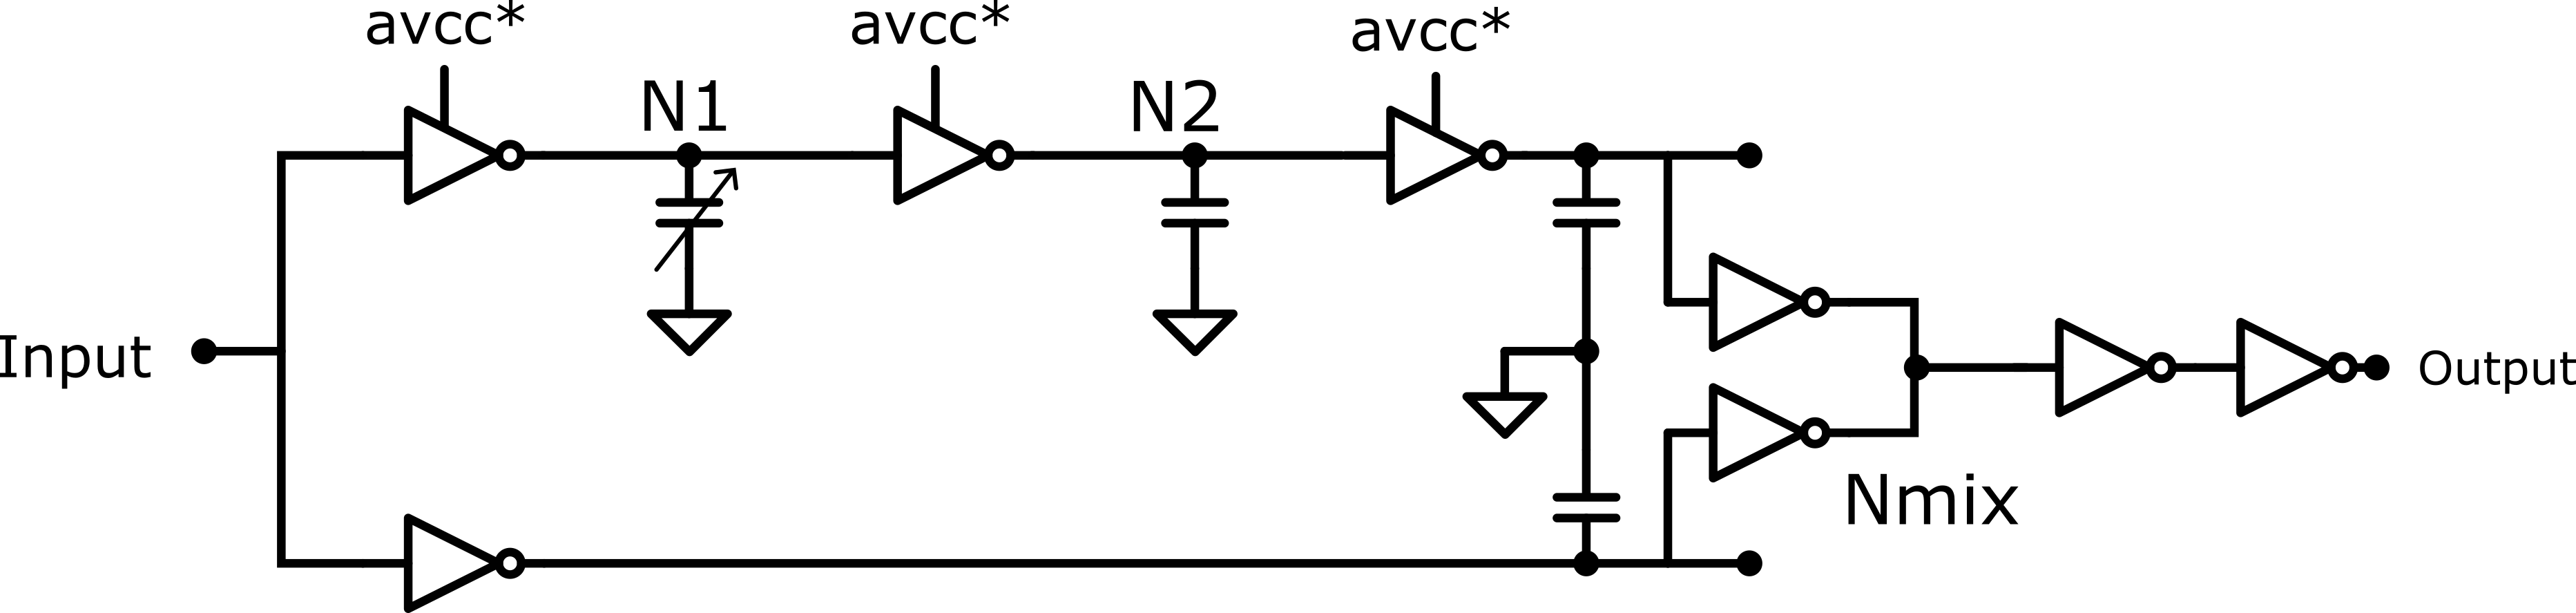
\includegraphics[width=0.8\linewidth]{figures/Schematics/clock_generation_half_V0.png}
  \caption{Phase interpolator with tunable capacitance and supply biasing.}
  \label{fig:PI_1_schematic}
\end{figure}

The resulting mixed-amplitude waveform is then passed through a final inverter, which has its own individually addressable supply, and a subsequent buffer that restores a full rail-to-rail swing, allowing for \gls{dcd} correction. This final stage effectively converts the voltage/amplitude modulation into a time-domain phase shift. Detailed derivations linking edge slew rate to duty-cycle variation and modelling the delay introduced by additional capacitance are provided in Appendix~\ref{app:duty_cycle_derivation} and Appendix~\ref{app:ln2_derivation}. In essence, a fractional increase in the rising-edge slew rate produces a proportional duty-cycle shift, while each added unit of capacitance introduces a fixed delay step.

By selecting appropriate combinations of $(C_\text{code},\Delta V_\text{DD})$, the circuit could achieve the required phase shift at the \ang{90} output. However, unequal rising and falling slew rates at the mixing node stemming from the voltage-tuning remained a significant source of error, necessitating the development of edge-balancing techniques.

\subsection{Duty-Cycle Correction Techniques}\label{sec:dcc}

Early prototypes of the phase interpolator exhibited a \gls{dcd} of approximately 7\% on the slow path. The following countermeasures were evaluated to mitigate this issue:

One option was to reduce the capacitive load at node $N_2$ (the output of the final delayed inverter). This was done to more closely match its rising and falling edge rates with those of the fast path, resulting in a noticeable but insufficient improvement in DCD.

Stacked-device inverters were also explored; Appendix~\ref{app:supp_figures} shows the topology (Fig.~\ref{fig:stacked_inv}). The standard \gls{ulvt} inverters were replaced with inverters featuring two-transistor stacked pull-up and pull-down branches. The symmetric series resistance of this stacked topology improved edge matching and significantly lowered DCD, albeit at the cost of increased device area and higher switching power. Introducing more devices into the design would also predictably increase noise and jitter, which was not acceptable for the target application, especially considering the mixing node was already a major contributor to jitter.


\subsection{2-stage Supply-Bias Fine-Tuning Variant}\label{sec:avcc_finetune}

Another variant of the PI (Appendix~\ref{app:supp_figures}, Fig.~\ref{fig:PI_2_schematic}) was developed where only the first two inverters in the delayed branch were voltage-tuned. By tuning an even number of inverters, the duty‑cycle distortion induced by each stage would partially counteract one another. Key observations from this variant were that adjusting the local supply \texttt{AVCC} over a \SI{\pm45}{\milli\volt} window changed the \ang{90} phase by approximately \ang{13}, representing a significant improvement compared to the \ang{4} range of the original three-inverter tunable path. Additionally, across the same bias range, the duty-cycle distortion improved from approximately 7\% to 2\%.

These results were positive and indicated that the supply-bias fine-tuning approach could provide a means of achieving the required phase shifts with reduced \gls{dcd}. However, \gls{dcd} remained a concern, as it was still too high for the target application and would necessitate the addition of further correction circuitry to ensure the output clock met the stringent requirements of the \gls{serdes} system. Since jitter was a critical parameter in the overall SerDes transmission chain budget, the team decided to explore alternative methods for achieving the required phase shifts without introducing significant \gls{dcd}, and possibly correcting the \gls{dcd} without additional stages.


\subsection{Current‑Starved Inverter Fine Tuning (Revisited)}\label{sec:csi}

To decouple the fine-tuning mechanism from induced DCD, a current‑starved inverter (\gls{csi}) was reintroduced into the design (Appendix~\ref{app:supp_figures}, Fig.~\ref{fig:PI_csi_schematic}). The \gls{csi} was placed as the second inverter in the \ang{90} branch, a location chosen because its output drives a smaller capacitive load, thereby maximizing the tuning resolution. The bias voltages $v_\text{bp}$ and $v_\text{bn}$ steer the pull‑up and pull‑down currents, respectively. A \SI{45}{\milli\volt} sweep of $v_\text{bp}$/$v_\text{bn}$, driven by a DAC with a \SI{3}{\milli\volt} step, resulted in phase shifts of \SI{35}{\femto\second} at the \ang{90} output. Critically, duty‑cycle distortion remained within 1.2\,\% across the tuning range.


\subsection{Phase interpolation challenges}\label{sec:PI_challenges}

A fundamental challenge with phase interpolation is that it requires the rising and falling edges of the signals being mixed to be slowed down significantly. For generating a \ang{90} out-of-phase clock, the rising and falling edges must overlap sufficiently to ensure correct mixing and avoid intermediate voltage plateaus as depicted in appendix~\ref{app:supp_figures} (Fig.~\ref{fig:fast}). This imposes a strict constraint on the signal rise/fall times. 

\subsubsection{Edge‑Overlap Constraint and Its Consequences}

Phase interpolation (PI) mixes two phase‑shifted clocks, e.g.\ $0^{\circ}$ and
\ang{90}, to synthesise an intermediate phase.  To obtain a clean
rail‑to‑rail output, the rising (or falling) edges of the two inputs must
overlap long enough that the resistive (or current‑mode) summer sees
both voltages simultaneously \cite{Razavi2023PI}.  For a data‑rate (or clock)
frequency $f$ the required rise/fall time is bounded by
%
\begin{equation}
{\;
     \frac{1}{4f+t_{\text{overlap}}} 
     \;<\; t_{\text{rise}} 
     \;<\; \frac{1}{2f}
     \;}
\label{eq:overlap}
\end{equation}
%
where the designer tries to maximise $t_{\text{overlap}}$ to minimise
mid‑rail plateaus (Fig.\,\ref{fig:fast} and Fig.\,\ref{fig:slow}).

\paragraph{Area penalty}:

The edge of a CMOS driver can be modelled as an \(R_{\text{on}}\)-\(C\) first‑order step.  
For the 10--90 \% definition of transition time,
\[
  t_{\text{rise}}\;\approx\;0.7\,R_{\text{on}}\,C_{\text{shunt}}
\]
Solving for the required shunt capacitance gives  
\[
  C_{\text{shunt}} \approx \frac{t_{\text{rise}}}{0.7\,R_{\text{on}}}
  \label{eq:C_shunt_area}
\]
Equation~\eqref{eq:overlap} constrains the rise time to
\(t_{\text{rise}}\gtrsim 1/(4f)\), therefore  
\[
  C_{\text{shunt}}
  \;\gtrsim\; 
  \frac{1}{\,0.7 \times 4\,f\,R_{\text{on}}}
  \;\propto\;\frac{1}{f}
  \label{eq:C_shunt}
\]
Because a Metal–Insulator–Metal capacitor obeys \(C\propto A\varepsilon/d\),
larger \(C_{\text{shunt}}\) directly means larger layout area.  
Hence the shunt–cap block becomes the dominant footprint of the PI slice as frequency decreases. 
Since the block had to work across frequencies, tuning for a large range of frequencies would likely require large, programmable capacitors, making the design less practical.

\paragraph{Jitter}:

Appendix~\ref{app:supp_figures} (Fig.~\ref{fig:slow}) removes the mid‑rail kink but forces the waveform to
linger near the inverter’s high‑gain point.  Treat the edge as a linear ramp
of height \(\Delta V = V_{\text{DD}}\) over
\(\Delta t = t_{\text{rise}}\), so
\(dV/dt \approx V_{\text{DD}}/t_{\text{rise}}\).
Any rms voltage noise \(\sigma_v\) present at that instant is converted into
timing jitter
\[
  \sigma_t
  \;=\;
  \frac{\sigma_v}{dV/dt}
  \;=\;
  \sigma_v \,\frac{t_{\text{rise}}}{V_{\text{DD}}},
\]
which increases linearly with \(t_{\text{rise}}\)
\cite{TektronixJitterPrimer2012}.  Using the 10--90\,\% definition would simply
replace \(V_{\text{DD}}\) by \(0.8\,V_{\text{DD}}\); the scaling remains
unchanged.

\ref{eq:C_shunt} and \ref{eq:C_shunt_area} reveal that, if the design is to delay phases through slew-rate adjustments, it is discouraged to slow down the edges more than strictly necessary, as this would increase the area and jitter.
% -----------------------------------------------------------

\subsubsection{Feed-forward technique}\label{sec:feedforward}
To overcome the aforementioned limitations of phase interpolation, a new feed-forward architecture (Appendix~\ref{app:supp_figures} (Fig.~\ref{fig:FF_half_1})) was proposed. This technique also utilizes internal nodes from two branches generating intermediate phase-shifted clocks but distinguishes itself by having a "master" and "slave" path, where the master drives an inverter that injects a current into the slave path. In other words, an internal tap from the faster signal path reinforces the slower one (or v.v.), causing the latter to settle at an intermediate phase. This method proved effective, operating with relaxed slew rate requirements at the internal nodes, making it a preferable alternative to the traditional PI design. It was stipulated that the feed-forward inverter should be programmable to allow for dynamic injection strength at the mixing node, so that both phases can be more independently controlled. As drawn in Appendix~\ref{app:supp_figures} (Fig.~\ref{fig:FF_half_1}), the mixing occurs before the signals are \ang{90} out of phase, thereby relaxing the slew‑rate requirements.


Appendix~\ref{app:supp_figures} (Fig.~\ref{fig:FF_half_Verilog-A_tuning}) shows the Verilog-A block tuning the feed-forward implementation. The capacitance coarse steps followed by fine-tuning the bias voltages of the current-starved inverter (\gls{csi}) are clearly identifiable as phase shift steps in the output clock over time.


\subsection{8-phase generation using feed-forwarding}\label{sec:8phase_FF}

Extending the three-output feed-forward architecture to an eight-output implementation introduced new challenges. Specifically, the initial strategy for generating the \ang{135} and \ang{315} phases proved ineffective. The feed-forward path from phase \ang{0} into the \ang{135}/\ang{315} branches, where the delay between internal nodes was still less than \ang{90}, resulted in the mixing of signals that were nearly \ang{135} or \ang{180} out of phase, rather than the intended \ang{45} or \ang{90}.

This issue was resolved by restructuring the mixing topology (Appendix~\ref{app:supp_figures}, Fig.~\ref{fig:FF_8out}). Instead of feeding forward from phase \ang{0}, the design was modified to mix phases \ang{270} and \ang{90} into the paths for \ang{0} (\ang{360}) and \ang{180}, respectively. Additionally, the tunable feed-forward inverters proved unnecessary, complicating the design while having negligible impact on the mixing quality. Concurrently, the inverters driving the \ang{0} and \ang{180} phases were deliberately weakened. The engineered strength imbalance between the two driving inverters further enhances the mixing behavior since the \ang{270} signal already experiences significant delay from multiple buffering stages, arriving at the mixing inverter with weakened drive strength. This configuration is more accurately described as a "feed-backward" approach, as it involves signals from later phases accelerating the transitions of earlier ones, though it is still referred to as feed-forwarding for consistency with the original architecture.


\subsection{3 nm Porting}\label{sec:3nm_porting}

Following its successful implementation in 7\,nm, the 8-phase feed-forwarding architecture was ported to a 3\,nm technology node. This was necessary to meet the higher target frequency of 22.5\,GHz, which was unattainable with the 7\,nm design. The porting process involved adapting the design to the new technology's characteristics, including transistor sizing and capacitance values.

The ported design retained the core feed-forward architectural principles. However, adjustments were made to account for the different properties of the 3 nm transistors, such as threshold voltages and drive strengths, and the tuning mechanisms were recalibrated. Jitter performance was verified using both transient and periodic noise (pnoise) simulations. After establishing a correlation between the two methods and adjusting simulation parameters, pnoise analysis was used exclusively for faster verification.

The initial 3\,nm design failed to meet jitter specifications, which necessitated doubling transistor sizes. While the capacitance and bias voltage tuning blocks successfully tuned the phases across \gls{pvt} variations, it was noted that the minimum capacitance of the MOS capacitor banks was higher than desired. This led to a reduction of most static capacitances in the circuit to compensate for this effect. The purpose of static capacitanes had been to provide a fixed delay shift in designs where the range of the tunable capacitors was sufficiently large, but consistently too low, meaning only the (e.g.) lower 70\,\% of the total available codes were being used. Higher frequencies, however, naturally required less total capacitance, and the static capacitances were not needed to achieve the required phase shifts. 

\subsection{Frequency range increase to 11~GHz - 22.5~GHz}\label{sec:freq_range}

The design was further adapted to operate across a wide frequency range from 11\,GHz to 22.5\,GHz. This required resizing the capacitor banks to ensure adequate phase shift control across the entire spectrum. This resizing led to an increase in the bank's total needed capacitance, which consequently increased the parasitic off capacitance as well.

The static capacitance values on most nodes were further reduced, in many cases to zero, making the capacitor banks the sole source of tunable capacitance, which was an unexpected yet positive design change. Importantly, a larger total capacitance also meant a larger step size, reducing the tuning resolution. However, the fine-tuning mechanism using current-starved inverters was able to compensate for this coarse resolution, although this required careful monitoring. In Figure~\ref{fig:FF_8out_CSI_dynamicTuning_PVT}, the Verilog-A tuning of the \ang{90} degree phase is shown, demonstrating the ability to dynamically adjust the phases across different \gls{pvt} corners and frequencies. For demonstrative purposes, some corners were chosen where the vb tuning was not sufficient to achieve the target phase, necessitating the recall of the coarse tuning block to adjust the capacitance code.

\begin{figure}[htbp]
  \centering
  \begin{subfigure}[t]{0.45\linewidth}
    \centering
    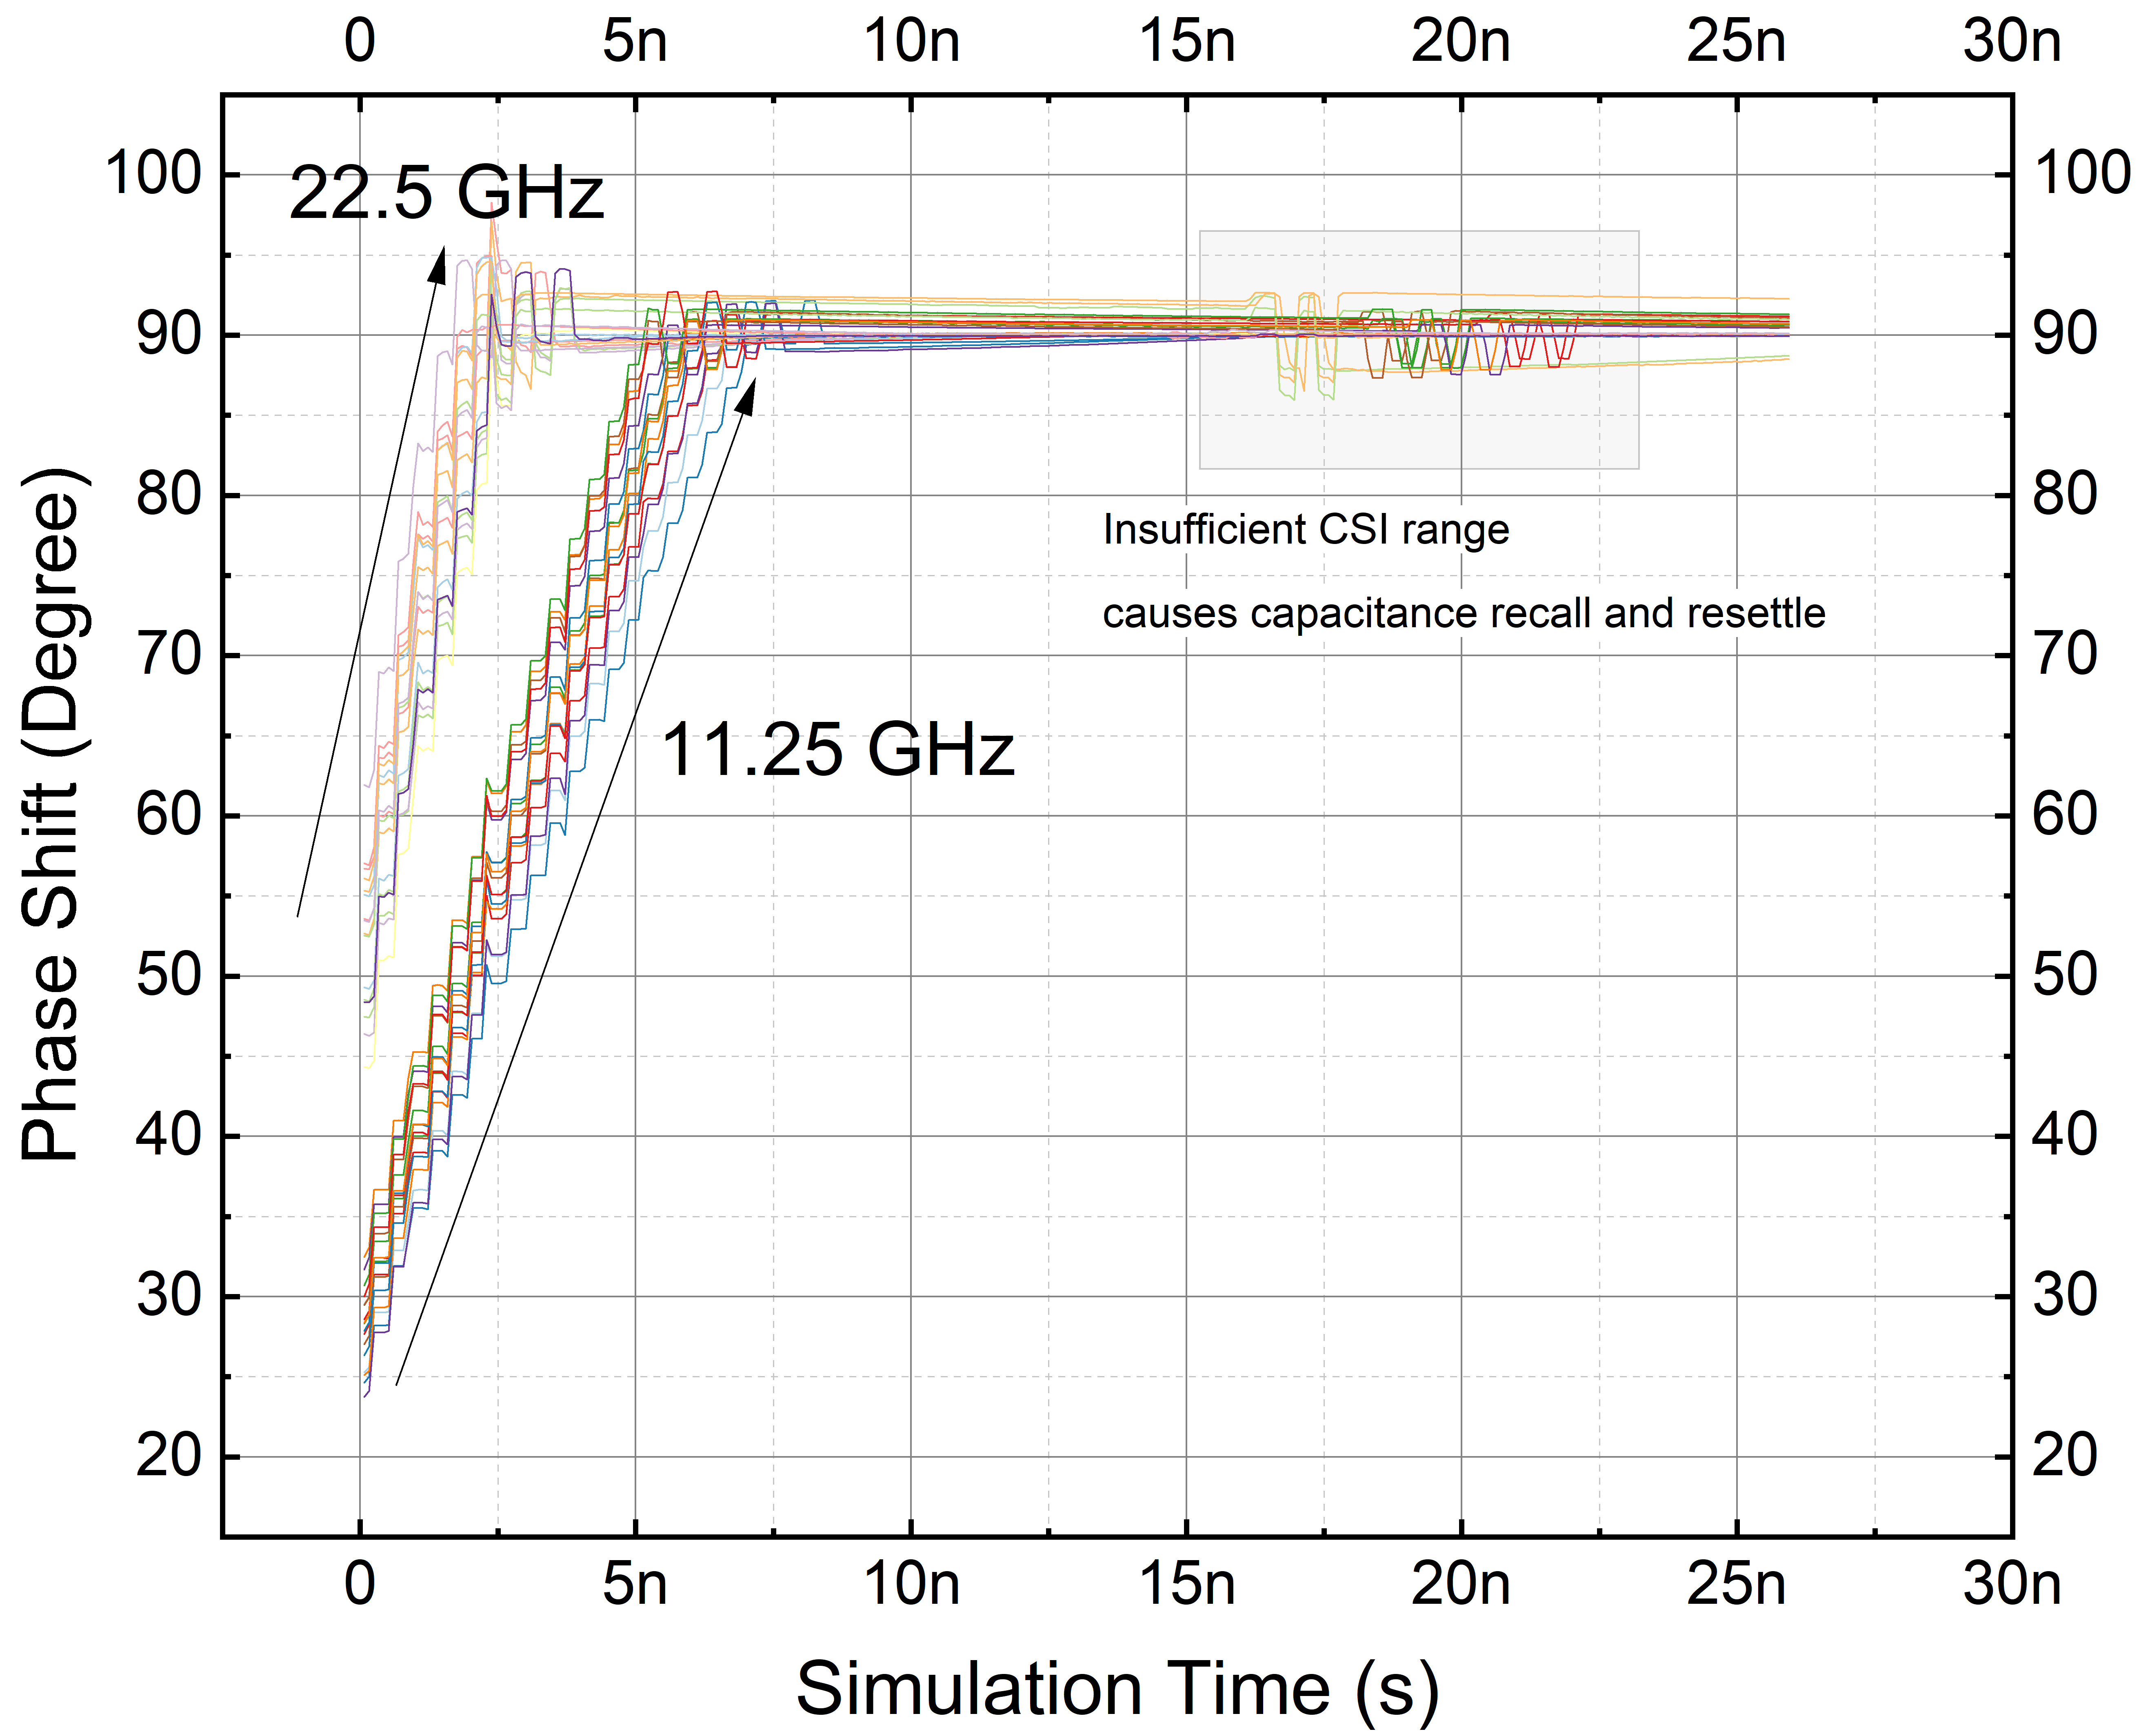
\includegraphics[width=\linewidth]{figures/Results/FF_8out_3nm_idealswitches-Phase90_tuning_PVT_SomeN.png}
    \caption{Verilog-A tuning of the 8-phase feed-forward architecture across different PVT corners. The coarse tuning block is recalled when the fine-tuning is insufficient to achieve the target phase.}
    \label{fig:FF_8out_CSI_dynamicTuning_PVT}
  \end{subfigure}
  \hfill
  \begin{subfigure}[t]{0.45\linewidth}
    \centering
    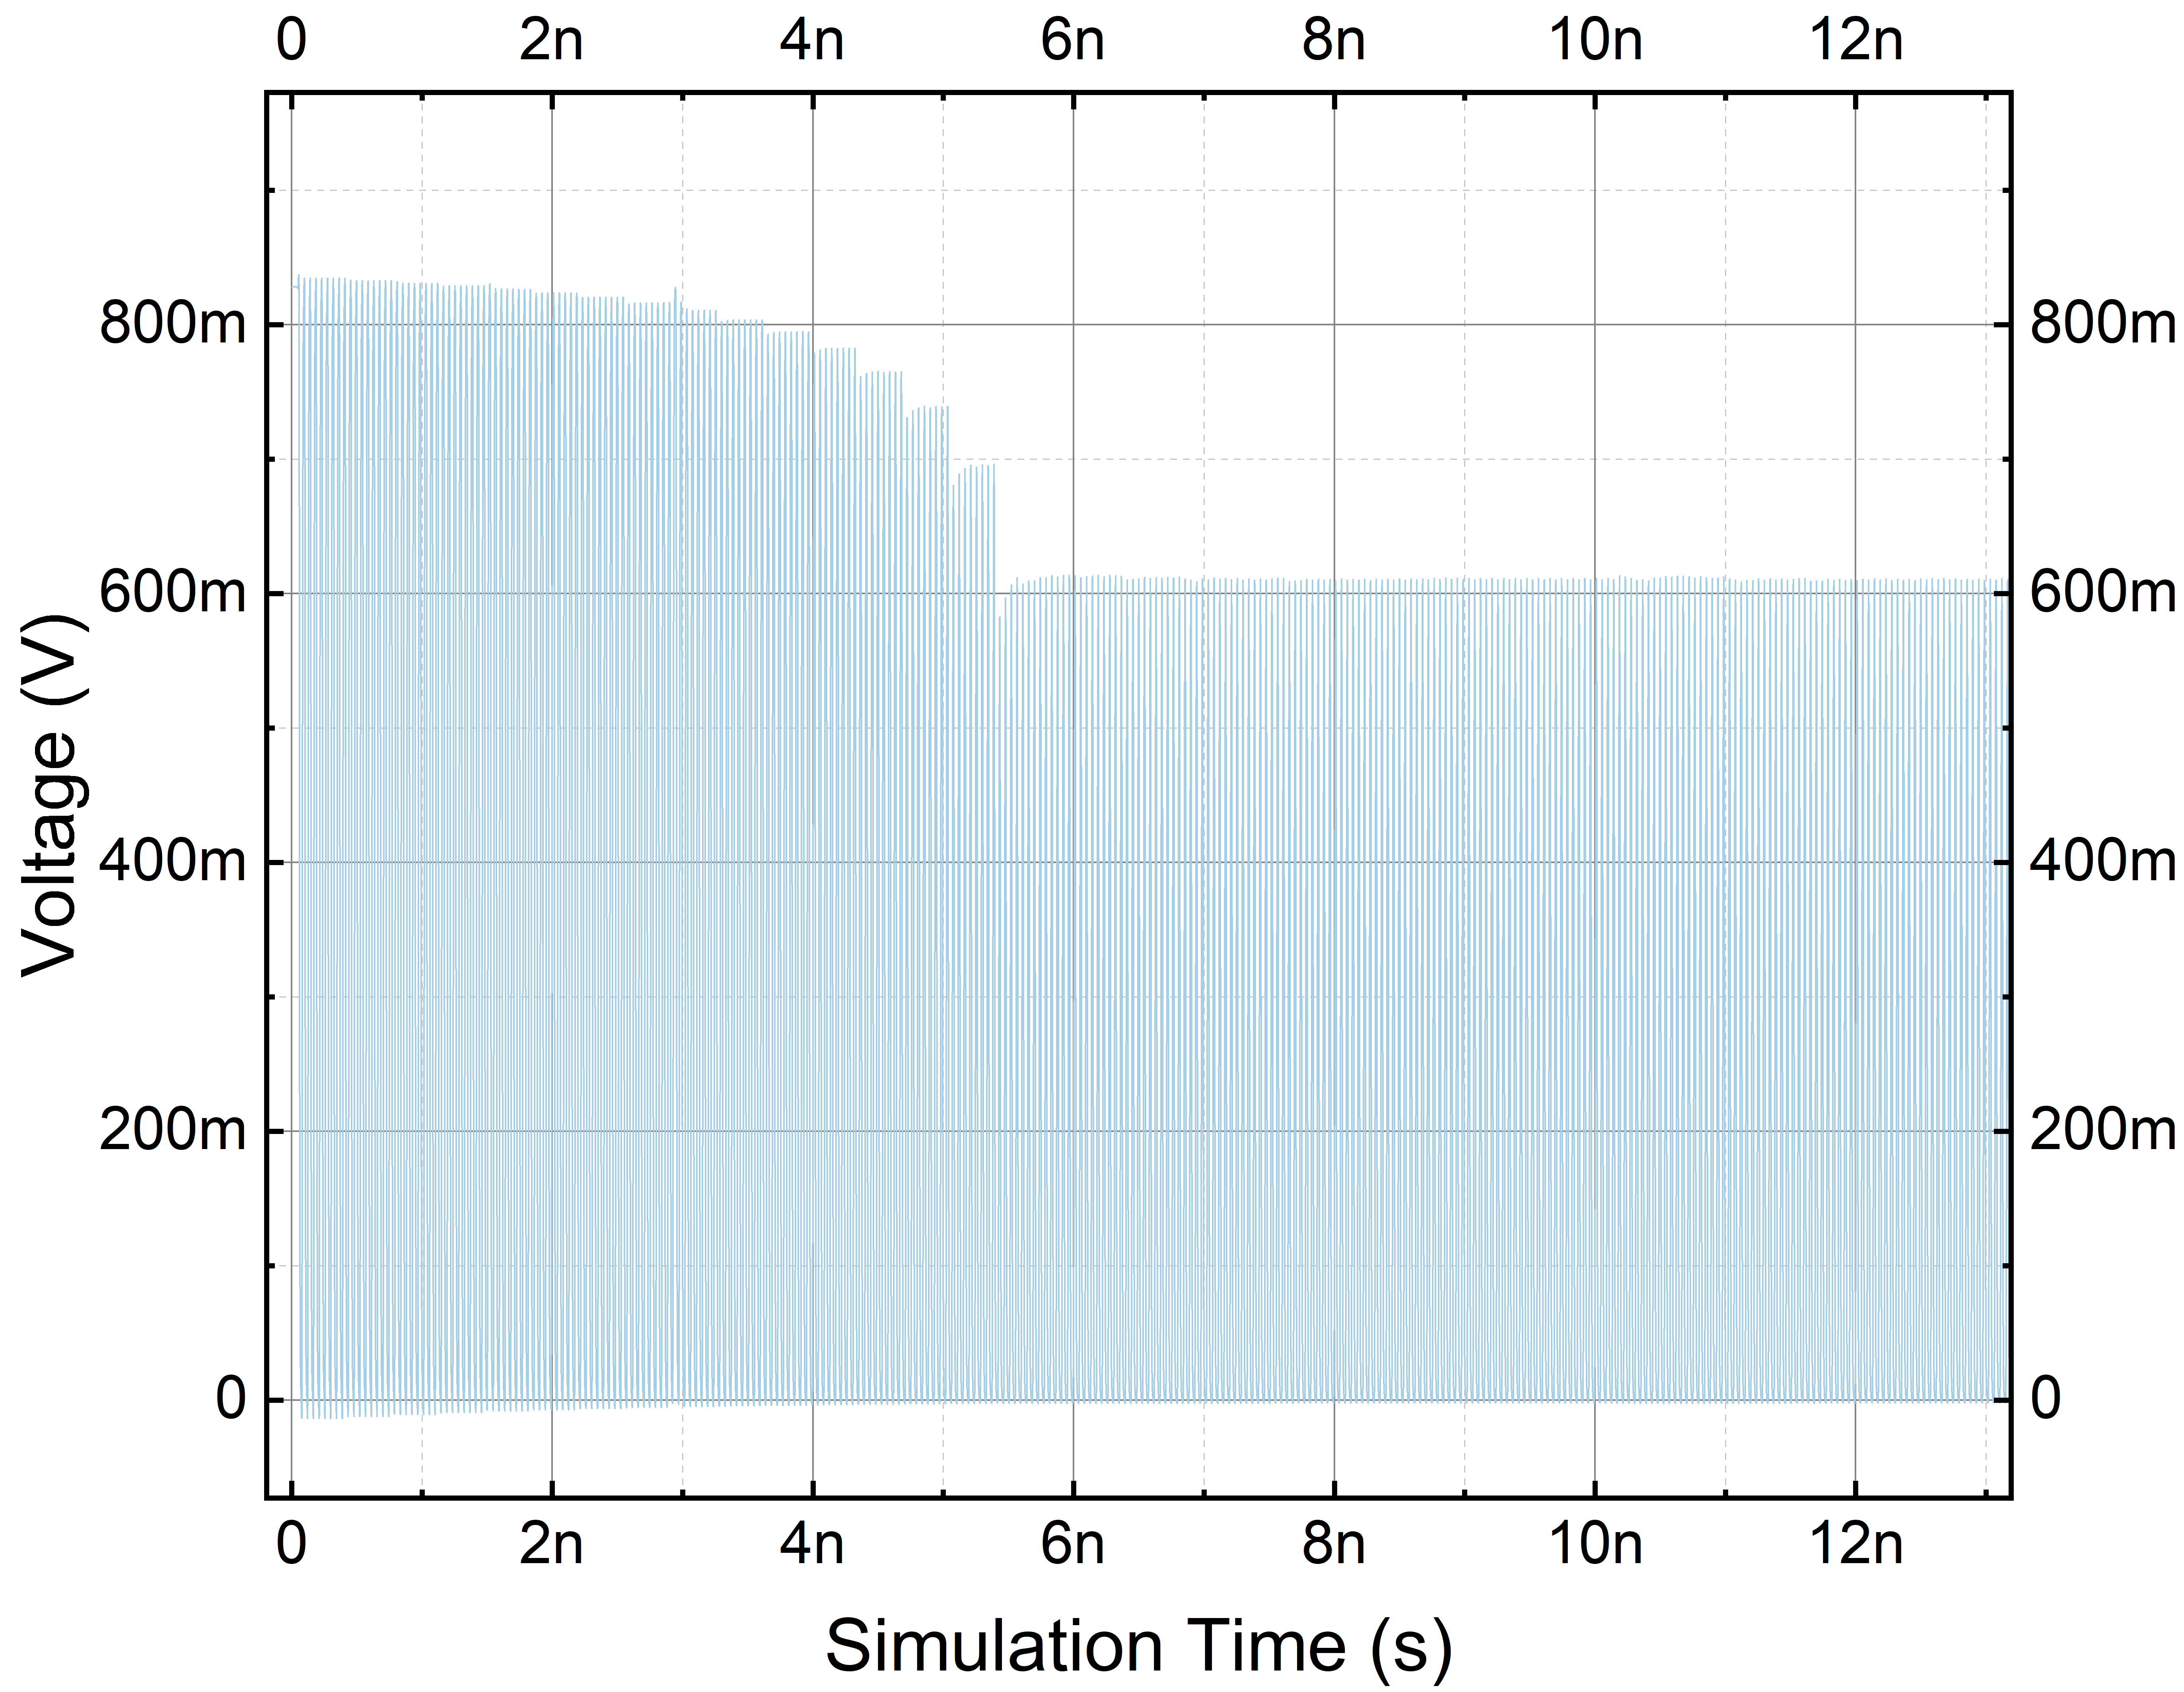
\includegraphics[width=\linewidth]{figures/Results/FF_8out_PPNN-DCDWithCap.png}
    \caption{Duty-cycle distortion caused by the voltage-dependent capacitance of the MOS-based capacitor bank. The wave mid-point is shifted away from half-supply, leading to a perceived DCD.}
    \label{fig:FF_CapDCD}
  \end{subfigure}
  \caption{Dynamic tuning and duty-cycle distortion in the feed-forward architecture}
  \label{fig:FF_tuning_and_dcd}
\end{figure}

\subsubsection{Capacitance bank behavior and duty‑cycle distortion}

It was observed that at lower frequencies (e.g., 11\,GHz), the higher total capacitance required for tuning unexpectedly caused duty‑cycle distortion. Investigation revealed that the capacitance of the MOS-based capacitor bank was highly dependent on the voltage of the node it was connected to. This voltage-dependent capacitance caused signals to have asymmetric rise and fall times, shifting the signal's crossing point away from half-supply and creating a perceived DCD.

This issue was mitigated by splitting the capacitor bank into two separate branches: one composed of NMOS transistors connected to ground, and another of PMOS transistors connected to VDD. Since the capacitance of an NMOS device increases with gate voltage while that of a PMOS device decreases, this dual-branch structure provides a more constant total capacitance across the signal voltage swing.

Three different dual-branch capacitor bank implementations were explored:
\begin{itemize}
    \item \textbf{"2P2N" Capacitor Bank:} What will hereafter be referred to as the "2P2N" capacitor bank (Figure~\ref{fig:2P2N_cap}) consists of an upper branch composed of a PMOS capacitor connected to the tap through a PMOS transistor, and a lower branch composed of an NMOS capacitor connected to the tap through an NMOS transistor. 
    \item \textbf{Tgate Capacitor Bank:} The "Tgate" capacitor bank (Figure~\ref{fig:Tgate_cap}) consists of a PMOS capacitor connected to the tap through a Tgate switch, and an NMOS capacitor connected to the tap through a second Tgate switch.
    \item \textbf{"PNPN" Capacitor Bank:} What will henceforth be called "PNPN" capacitor bank (Figure~\ref{fig:PNPN_cap}) consists of a PMOS capacitor connected to the tap through an NMOS transistor, and an NMOS capacitor connected to the tap through a PMOS transistor. The rational for this design is that the NMOS switch will more easily pull the voltage at the PMOS capacitor tap down, while the PMOS switch will more easily pull the voltage at the NMOS capacitor tap up. Since the PMOS capacitance increases with decreasing gate voltage, and the NMOS capacitance increases with increasing gate voltage, this design was expected to provide a more stable capacitance across the voltage swing. The secondary objective was to reduce layout complexity when compared to the Tgate capacitor bank.
\end{itemize}
All capacitor banks were designed as a binary-weighted array of the unit cells shown in Figure~\ref{fig:2P2N_cap}, \ref{fig:Tgate_cap}, and \ref{fig:PNPN_cap}. Both the MOSCap and the switches scaled in the same proportions to keep RC delays constant across codes. 


A testbench was set-up to compare the performance of these three capacitor banks. The switch transistors and MOSCap sizings were set to the same values across all three banks for consistency. All three designs were controlled by an ideal 5-bit digital control. The testbench measured the step sizes of each bank across a range of frequencies, as well as the off capacitance at code 5b'00000. Beyond this, the capacitance values were also compared across tap voltages to assess the voltage dependency of the capacitance.

Capacitance values were extracted by running an ac simulation and subsequently extracting the imaginary part of the impedance at the tap node. This is expressed by the frequency-dependent equation:
\begin{equation}
  C_{\text{tap}}(F) = \frac{1}{2\pi f \textit{Im}(Z_{\text{tap}})}
\end{equation}

The 2P2N and PNPN capacitor banks were found to be similar in terms of step sizes across codes, while the Tgate consistently provided larger step sizes. Moreover, the Tgate capacitor bank exhibited the highest off capacitance (roughly double that of the 2P2N and PNPN banks), which was expected since even when the switch was off, there were a higher number of transistors connected to the tap node, leading to a larger parasitic capacitance.
Across tap voltages, the 2P2N and PNPN capacitor banks exhibited the less consistent capacitance values, with the 2P2N bank still showing a significant improvement in capacitance stability across tap voltages. The Tgate capacitor bank showed the most consistent capacitance values across tap voltages, with a very small variation.
Figures \ref{fig:cap_vs_codes} and \ref{fig:cap_vs_tap_voltage} verify these observations, showing the step sizes across codes and the capacitance values across tap voltages for each capacitor bank, sampled at 22.5~GHz.

\begin{figure}[htbp]
  \begin{subfigure}[t]{0.45\linewidth}
    \centering
    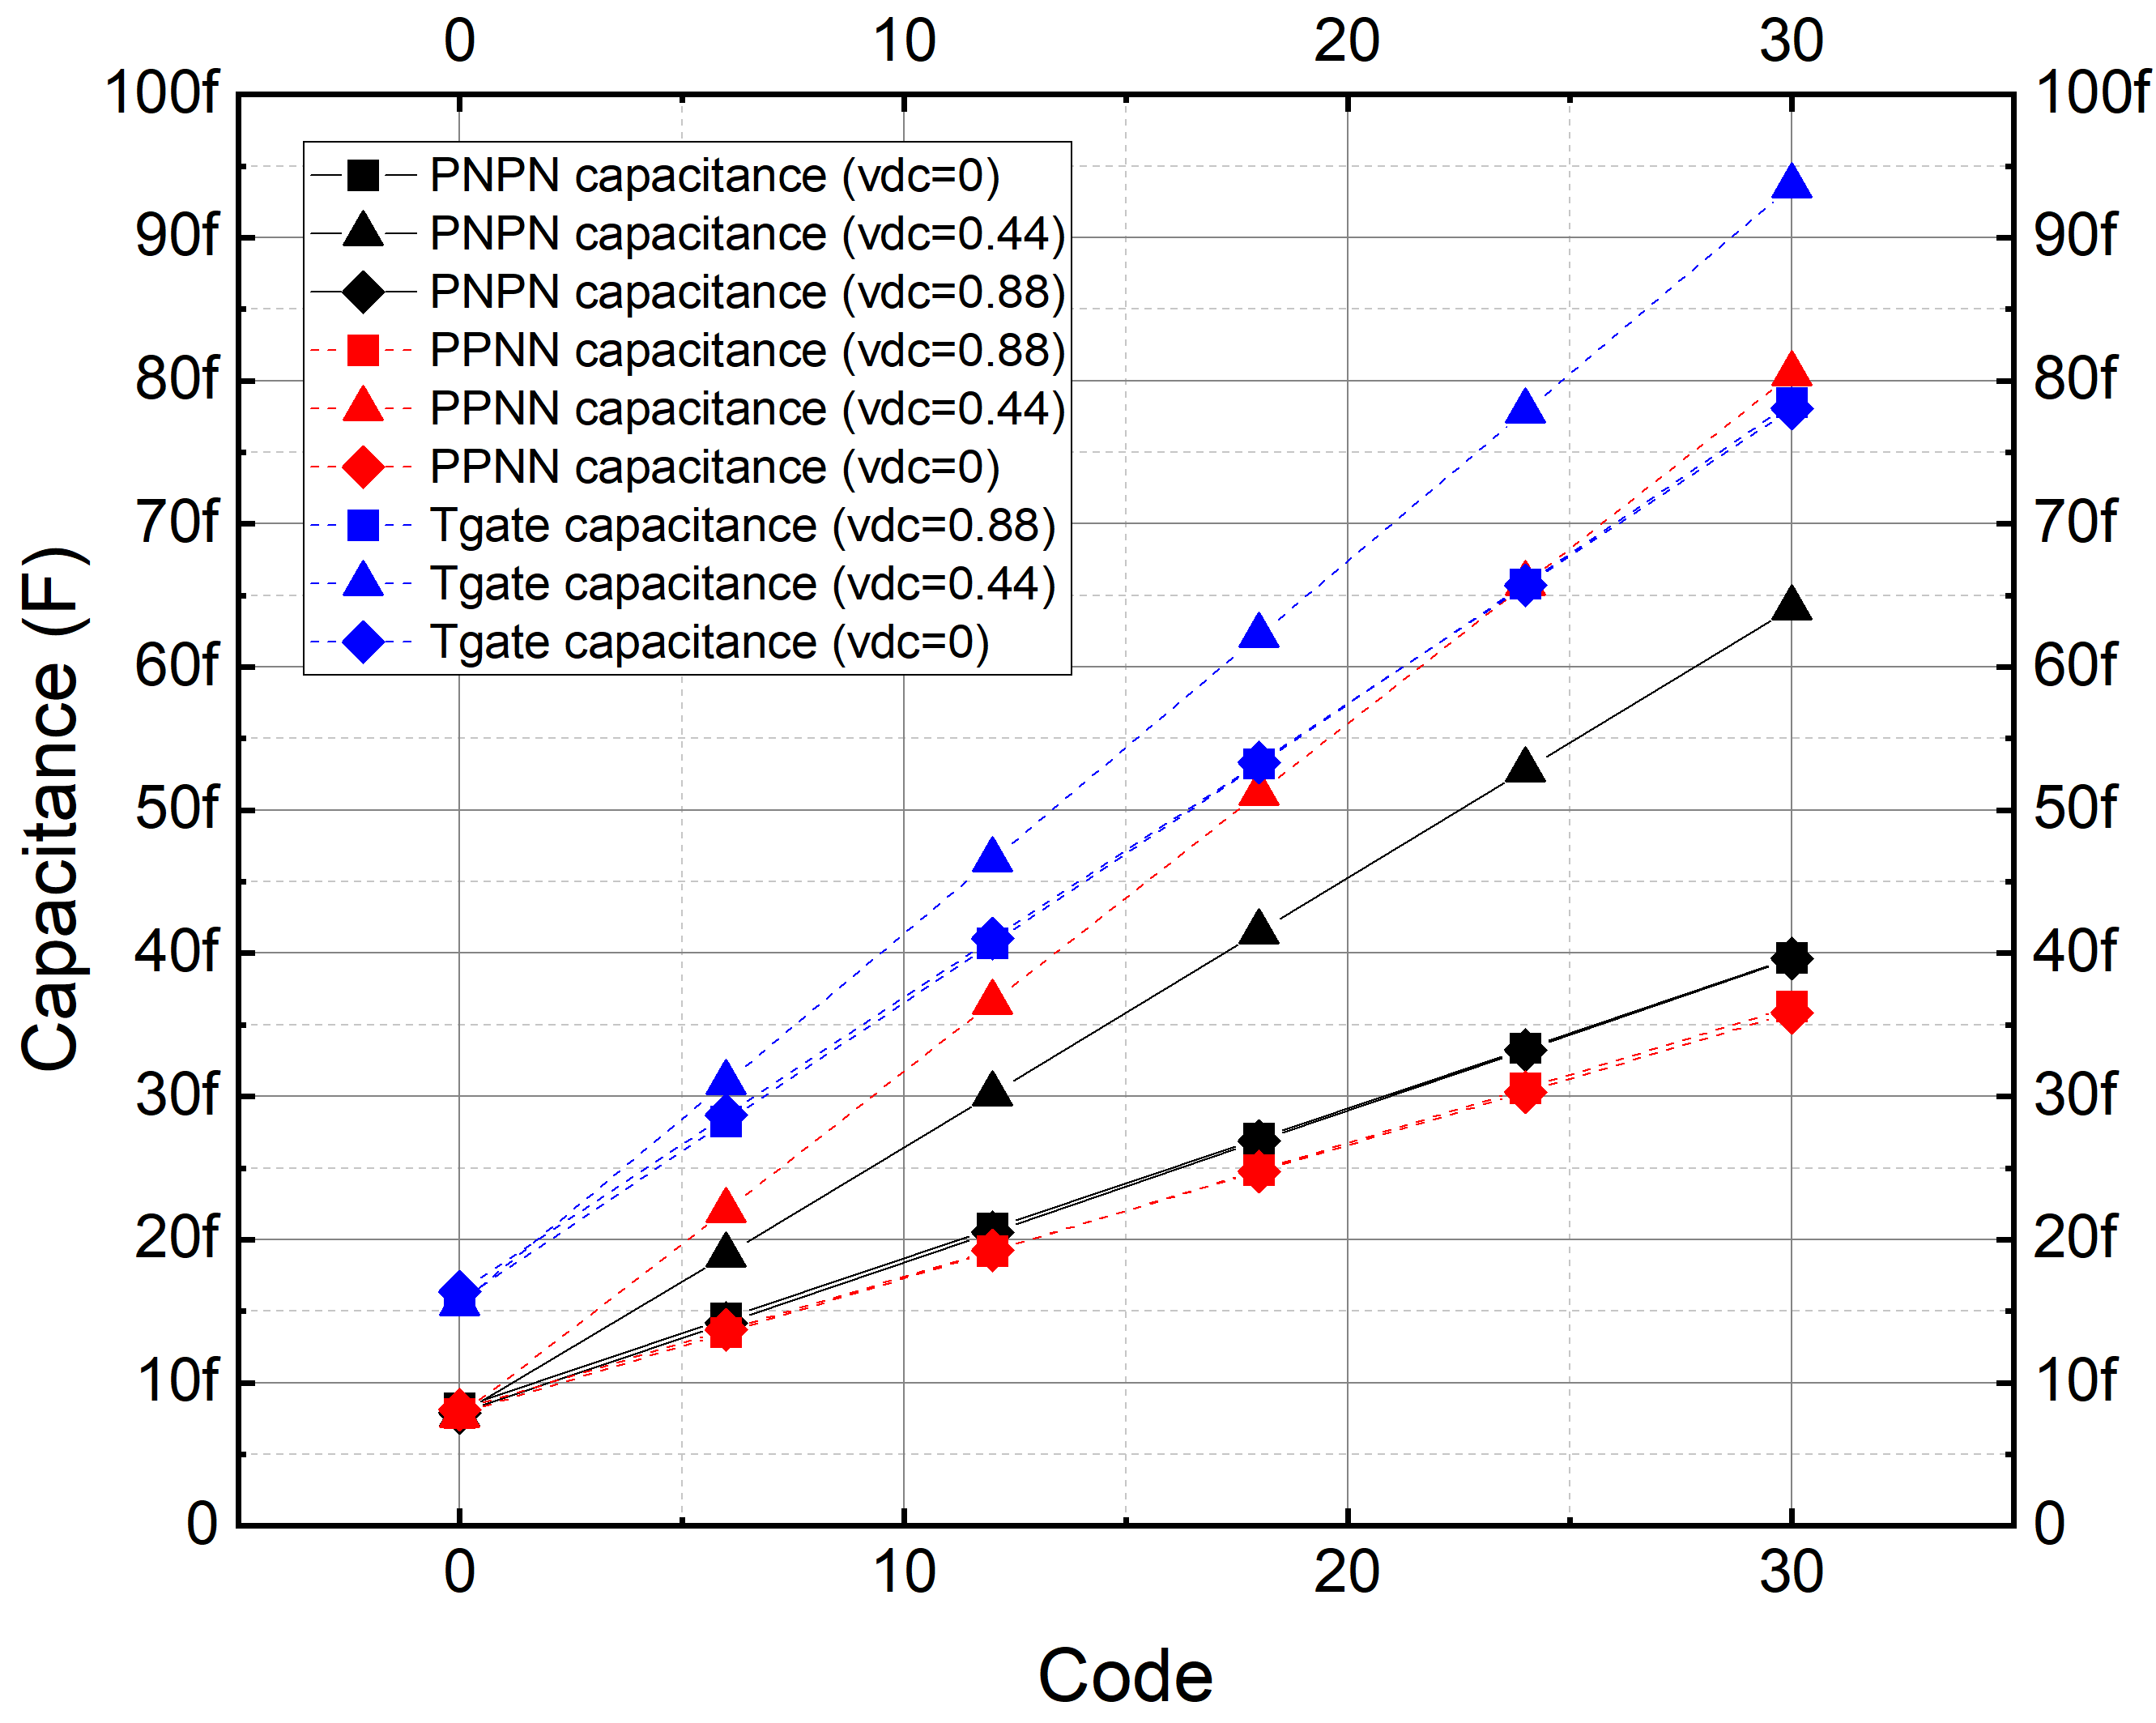
\includegraphics[width=\linewidth]{figures/Results/Cap_tests-CapVsCode.png}
    \caption{Capacitance step sizes across codes for the three capacitor bank implementations. The Tgate capacitor bank exhibits larger step sizes compared to the 2P2N and PNPN banks.}
    \label{fig:cap_vs_codes}
  \end{subfigure}
  \hfill
  \begin{subfigure}[t]{0.45\linewidth}
    \centering
    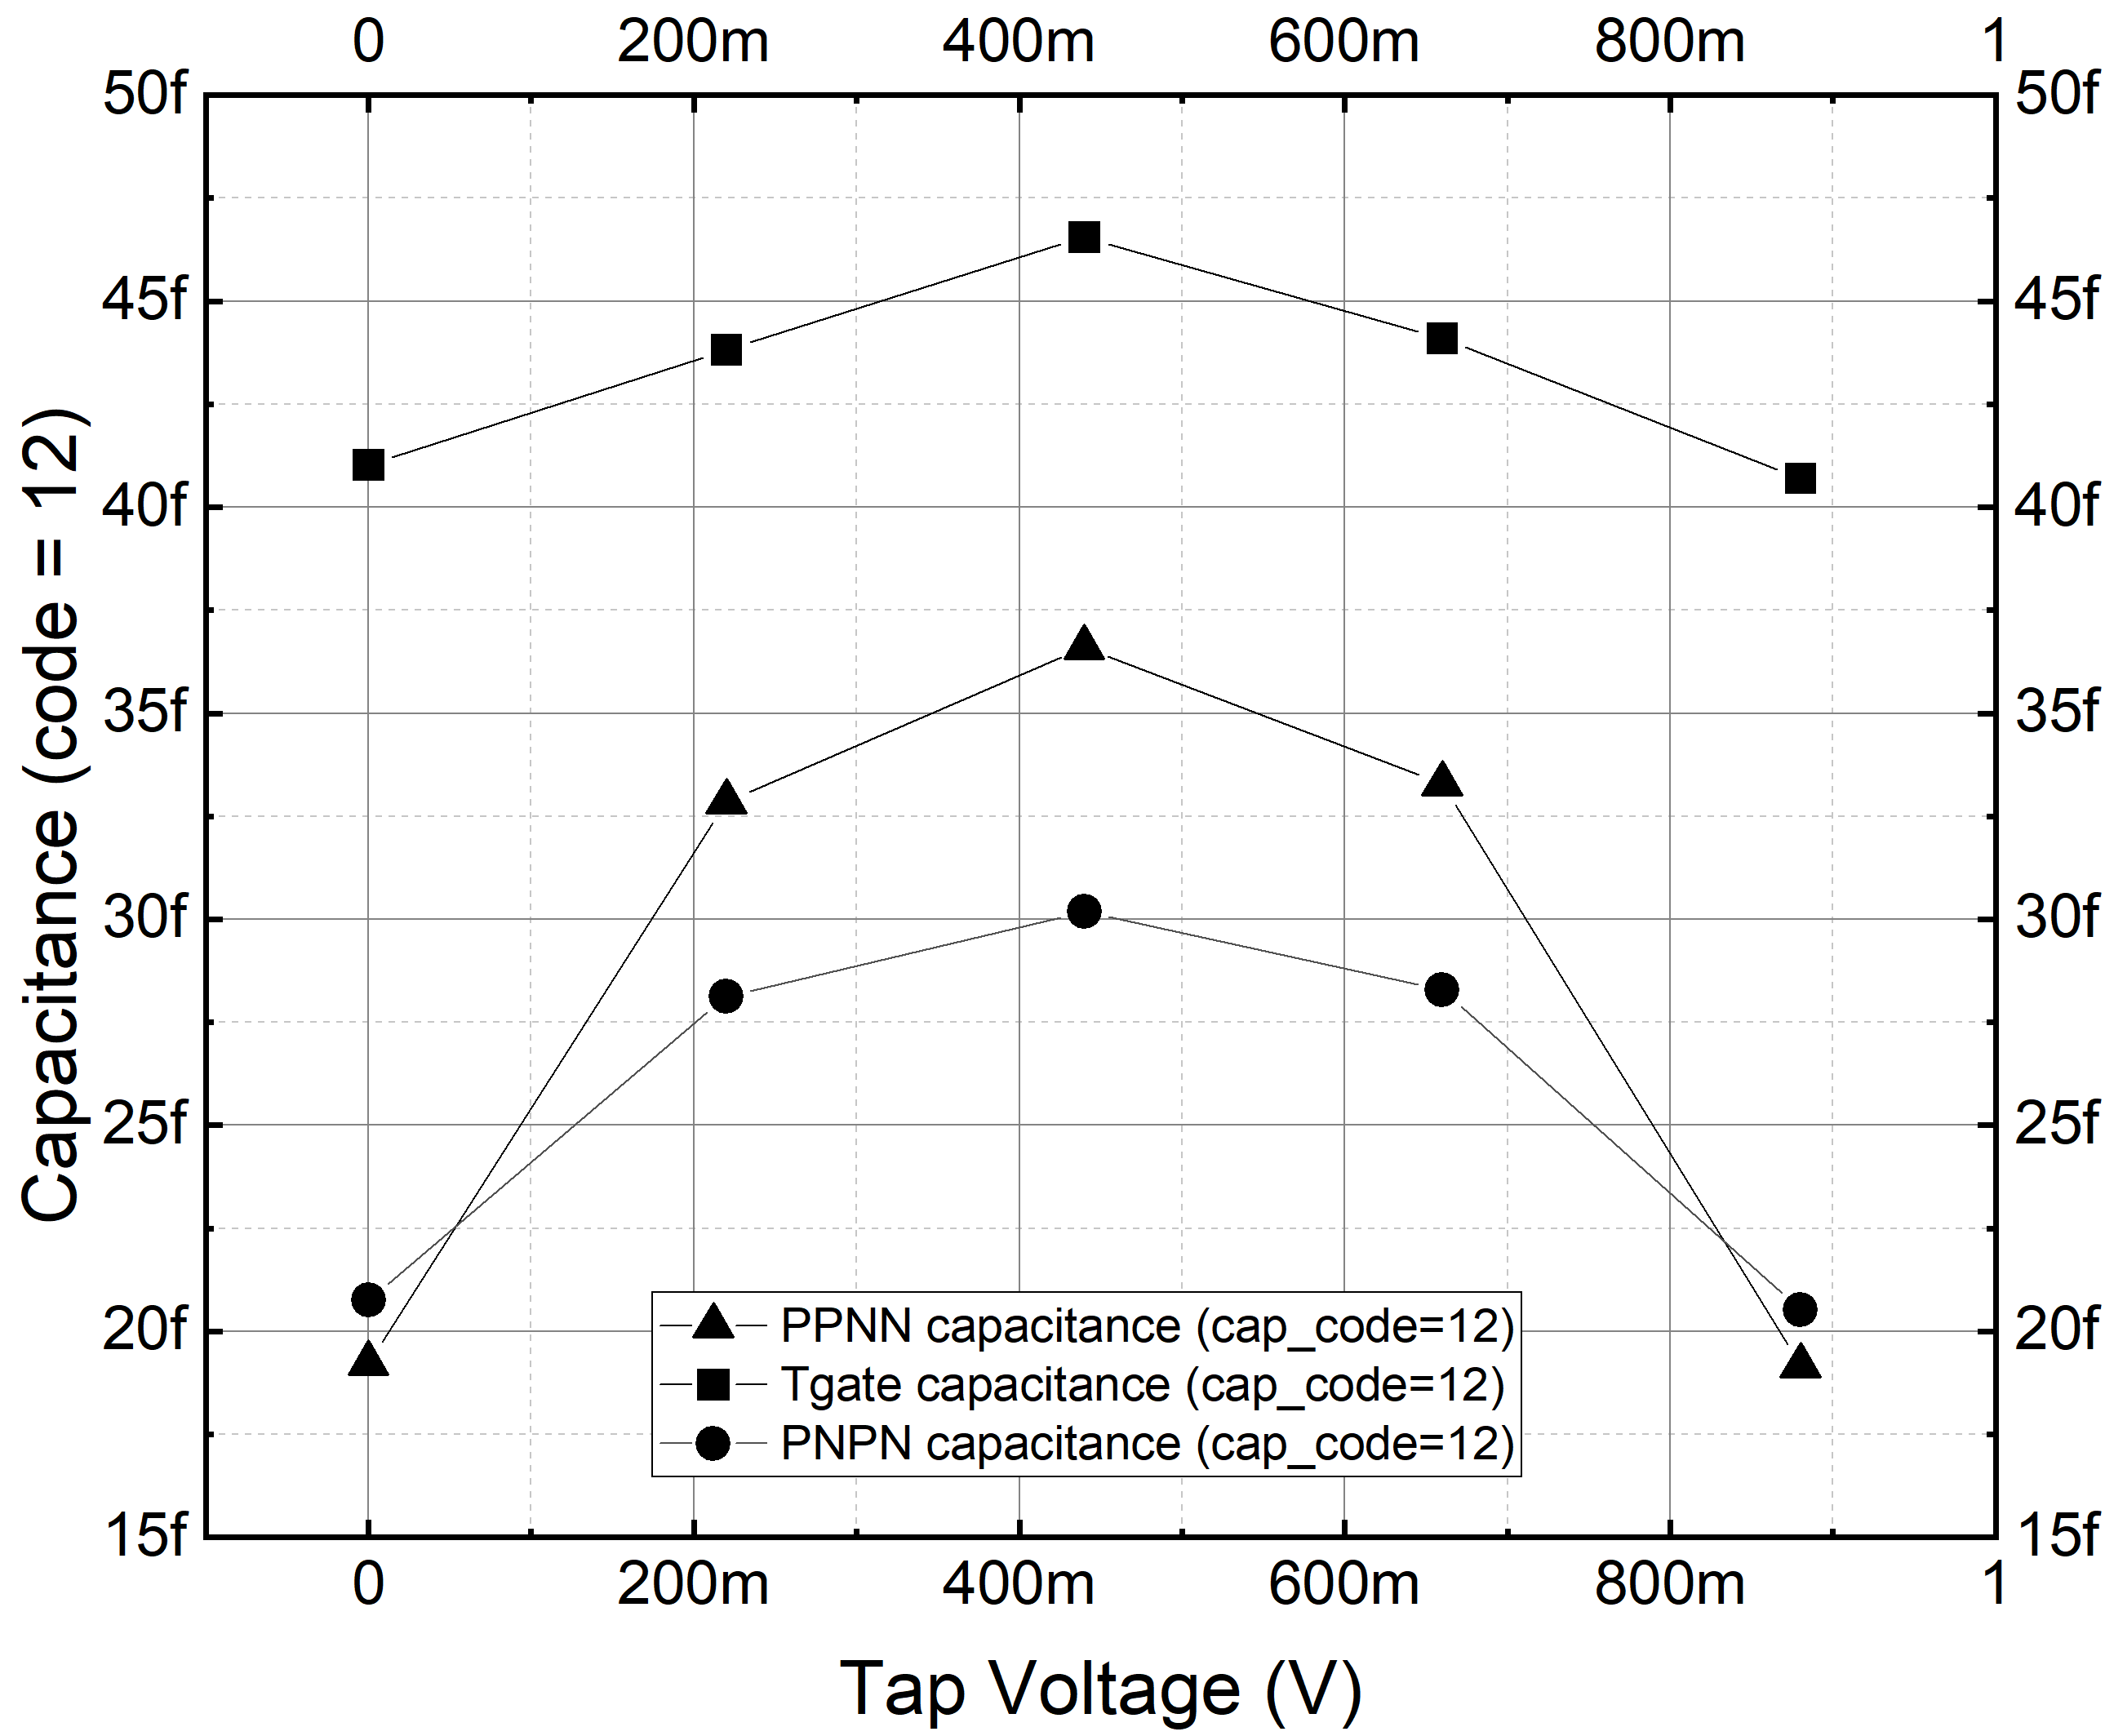
\includegraphics[width=\linewidth]{figures/Results/Cap_tests-CapVsVoltage.png}
    \caption{Capacitance values across tap voltages for the three capacitor bank implementations. The Tgate capacitor bank exhibits more consistent capacitance values compared to the 2P2N and PNPN banks.}
    \label{fig:cap_vs_tap_voltage}
  \end{subfigure}
\end{figure}

\subsection{Parasitic Back-Annotation Strategy}

To model post-layout behaviour we first back-annotated parasitic capacitances extracted with \textsc{ParagonX Pro}.%
The extracted values were inserted as ideal lumped capacitors between every relevant node pair (\(V_\text{IN}\), \(V_\text{OUT}\), \(V_\text{DD}\), \(V_\text{SS}\)) as drawn in Figure~\ref{fig:back_annotation}.

\begin{figure}[htbp]
  \centering
  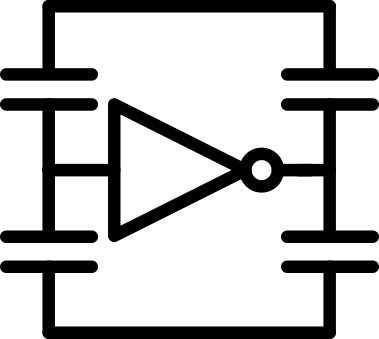
\includegraphics[width=0.15\linewidth]{figures/Schematics/BackAnnotation.png}
  \caption{Parasitic capacitances extracted with \textsc{ParagonX Pro} inserted as ideal lumped capacitors between every relevant node pair.}
  \label{fig:back_annotation}
\end{figure}

This initial experiment was performed on a simple buffer layout rather than the full 22.5 - 5~GHz multi-phase generator.
As a result, the reported parasitic caps were overly large and the back-annotated schematic failed at the target frequency: several clock phases collapsed or showed severe duty-cycle distortion across PVT corners.
Even with careful sizing of the MOS capacitors and switches, the parasitic load remained too high.
A second simulation was therefore carried out on a compact testbench.  
We compared i) the transient response of this post-layout netlist with ii) a schematic in which the extracted caps were multiplied by a global scaling factor.  
Good agreement appeared even when the scale factor was far below unity.  
Inspection of the DC operating point clarified the reason: the TSMC transistor wrapper models already include femtofarad-level capacitances beyond intrinsic and overlap capacitances that dominate most layout-dependent contributions at low metal levels.

Hence the wrapper-based schematic already mimics the bulk of the real parasitic capacitance.  
A fully accurate absolute back-annotation would require a specialised, fully optimised layout well beyond the exploratory buffer used here yet side-by-side comparisons show that the schematic plus wrapper reproduces post-layout behaviour closely enough for the current stage of the project.
It was thus decided that back annotation was not to be introduced at this stage, with an expected future revision to include a more accurate back-annotation of the parasitics, once the design is more mature and the layout is available.

\subsection{Redesign in favor of pure delay implementation}\label{sec:second_redesign}

Although the feed-forward implementation successfully generated the eight clock phases, it exhibited instability in phases \ang{135} and \ang{315} under certain process corners. This instability occurred when the delay requirements of different branches came into conflict. For example, in a fast-fast (FF) corner, the \ang{90}/\ang{270} paths might require increased capacitance to add delay, while the \ang{135}/\ang{315} paths might require reduced capacitance. Since \ang{90} feeds into \ang{135}, the two branches are coupled, and the tuning of one phase directly affects the other, meaning both branches were "fighting" to achieve their respective delays. Figure~\ref{fig:FF_8out_225vs135} illustrates this issue, where the \ang{135} is overcorrected as a consequence of the \ang{270} phase being too fast, leading to the former needing to decrease codes to achieve the desired phase shift.

\begin{figure}[htbp]
  \centering
  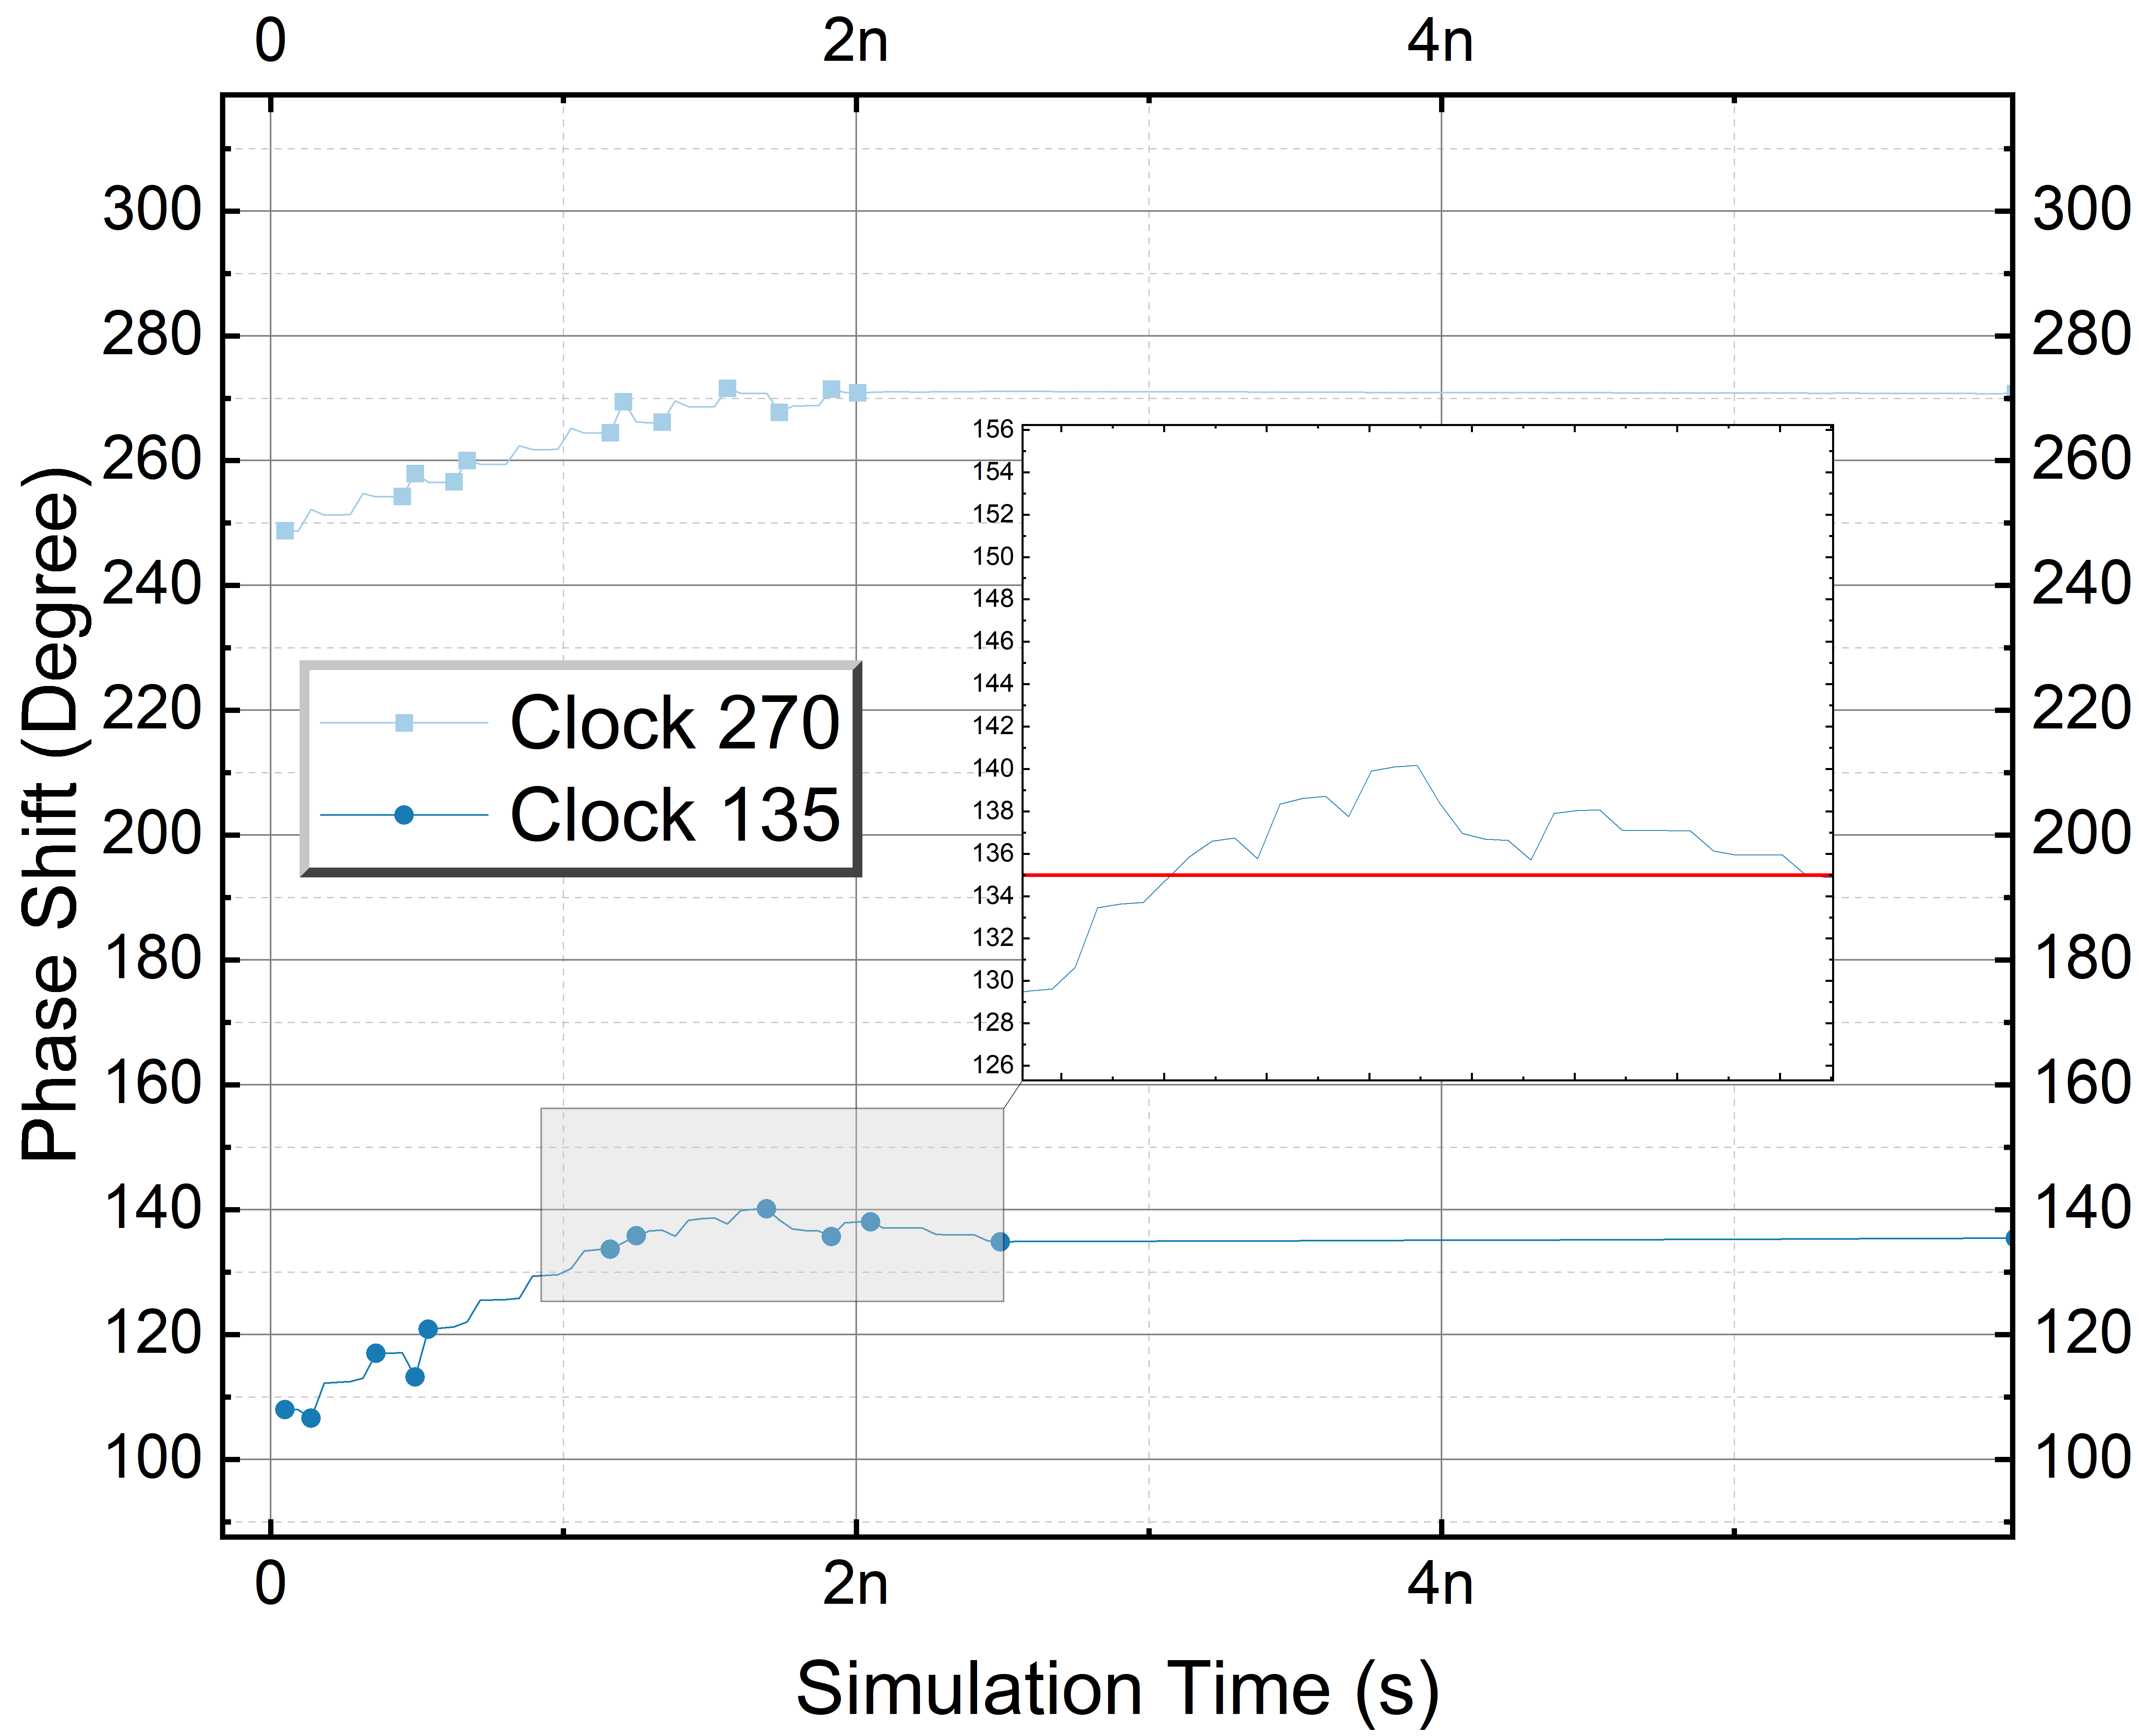
\includegraphics[width=0.6\linewidth]{figures/Results/FF_8out_PNPN-FightExample.png}
  \caption{Conflict between the \ang{270} and \ang{135} phases in the feed-forward implementation. The \ang{135} phase is overcorrected due to the \ang{270} phase being too fast, leading to a decrease in codes to achieve the desired phase shift.}
  \label{fig:FF_8out_225vs135}
\end{figure}

To address this fundamental issue, a second major redesign was undertaken, abandoning the feed-forward approach in favor of a pure delay implementation (Figure~\ref{fig:pure_delay}). This new architecture simplified the phase generation process by returning to a more traditional delay line structure, providing more consistent and, crucially, independent phase shifts for all eight outputs.

The new design retains eight independent delay paths but eliminates the feed-forward/backward mixing mechanism. Instead, it relies solely on a series of programmable delay elements within each path. This ensures that the tuning of one phase does not interfere with any other, resolving the stability issues observed with phases \ang{135} and \ang{315}.

\begin{figure}[htbp]
  \centering
  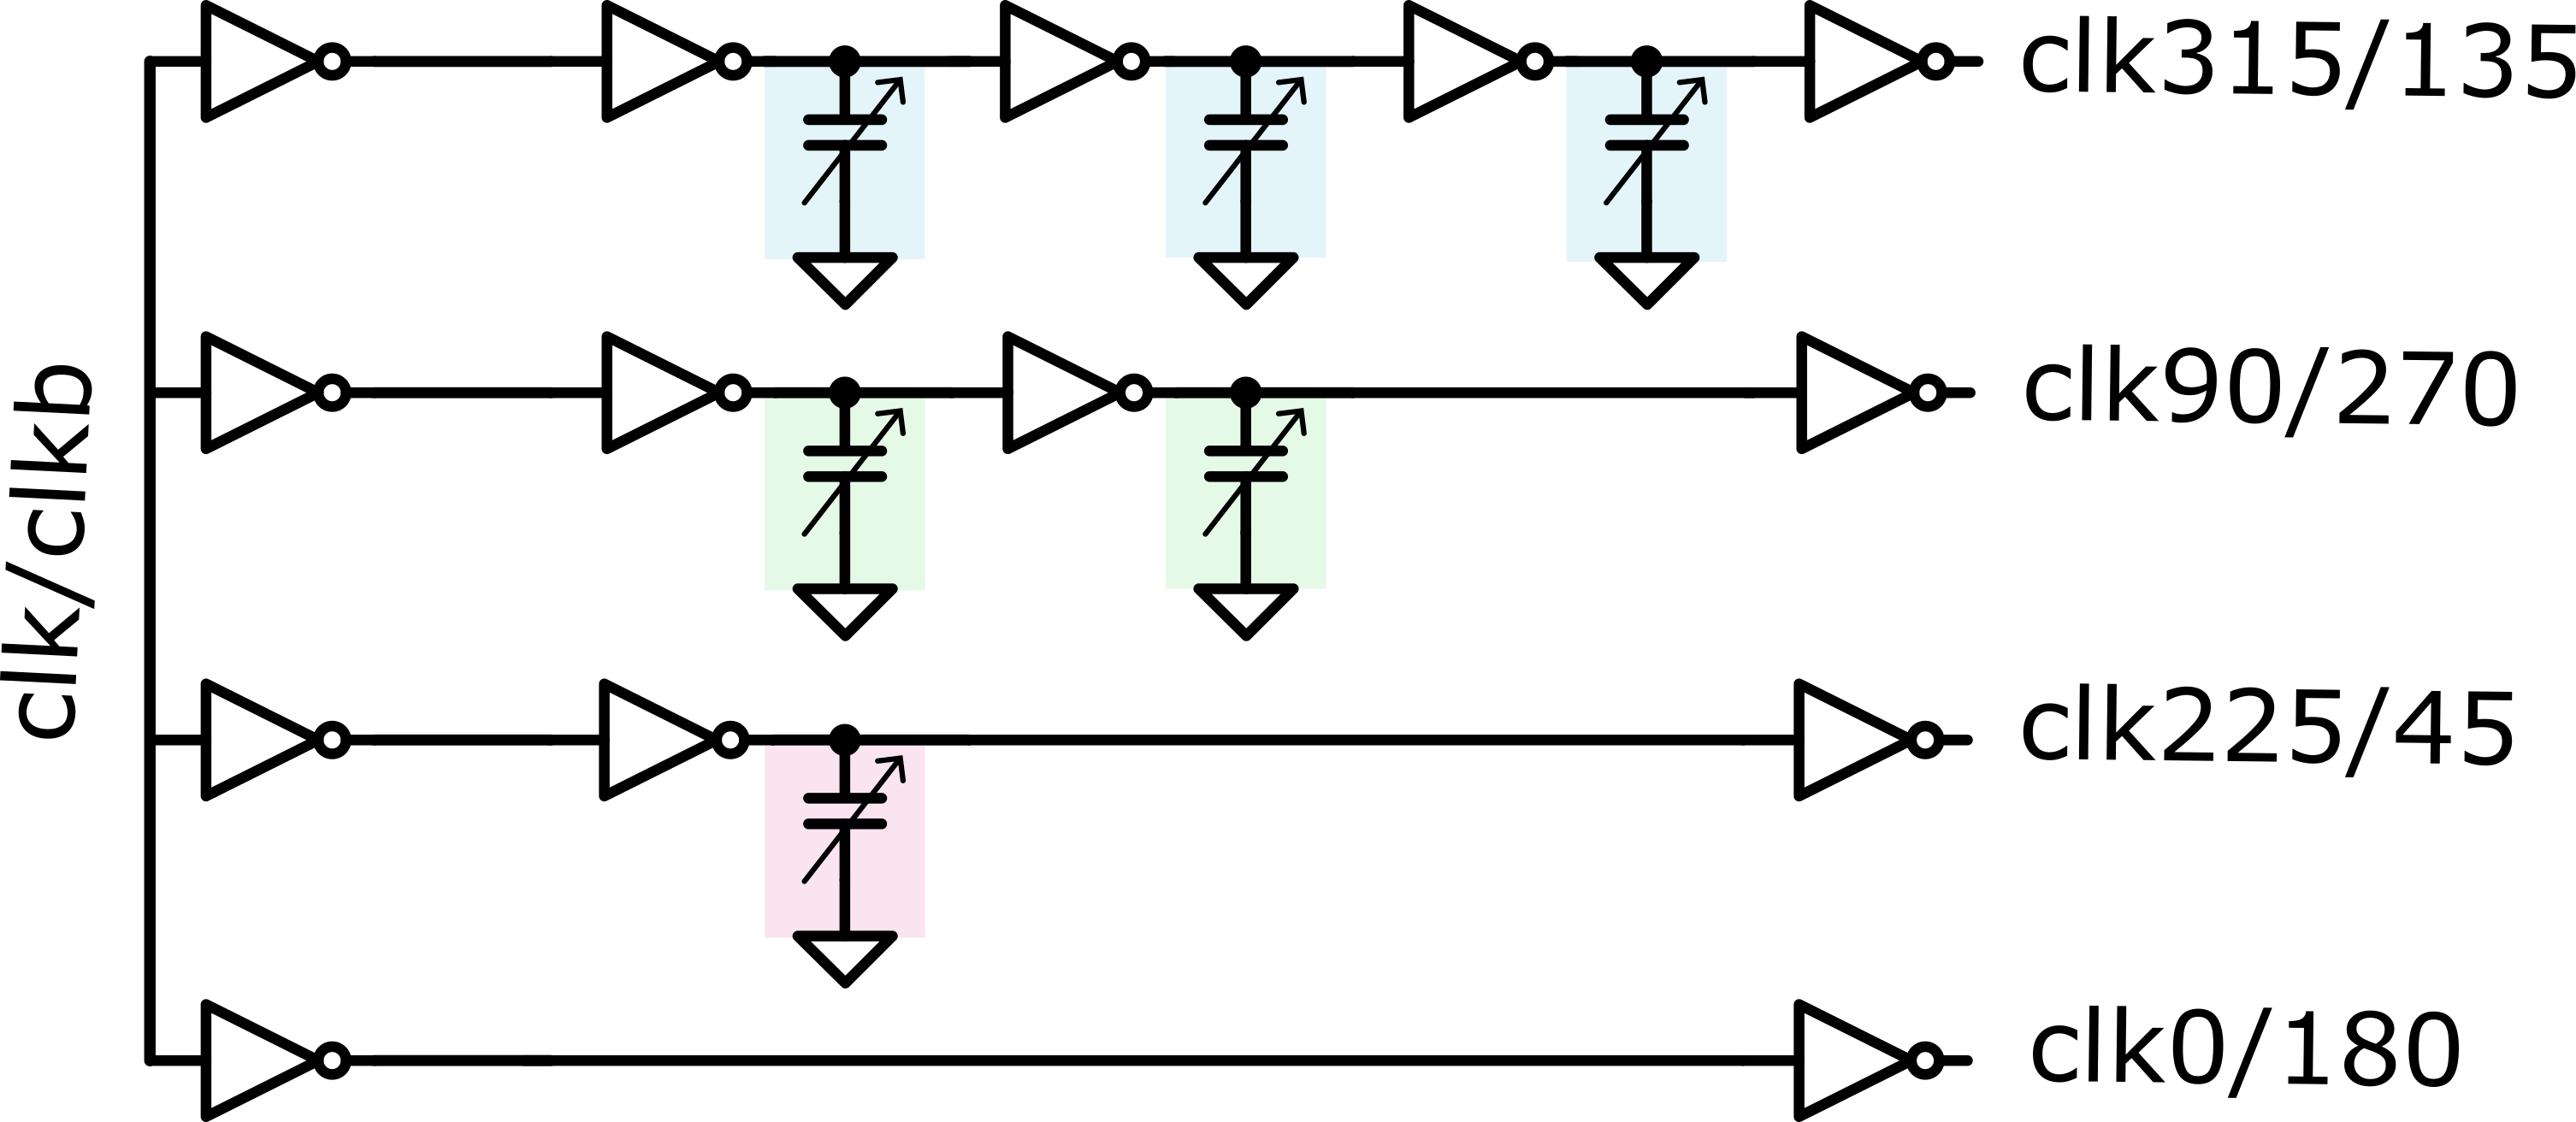
\includegraphics[width=0.7\linewidth]{figures/Schematics/pure_delay.png}
  \caption{Pure delay DLL architecture. Each of the eight phases is generated by a dedicated delay path, ensuring independent phase shifts and resolving stability issues observed in the feed-forward implementation.}
  \label{fig:pure_delay}
\end{figure}


Initially, a pure delay-line architecture had been discounted due to concerns about higher power dissipation and potentially worse jitter performance compared to the feed-forward design. While the power dissipation was indeed slightly higher, it was found that with careful design, the pure delay implementation could achieve comparable jitter performance.

A key observation was that spreading the required delay over a larger number of stages, each with a smaller capacitive load, led to lower jitter. This was attributed to two factors: 1) the improved slew rate of the less-loaded inverters, and 2) the increase of the low-pass cutoff frequency of each inverter stage, which improved the signal-to-noise ratio. As a result, every stage adds a delay of roughly \ang{45}, which results in phases \ang{315}/\ang{135} having a total of 5 cascaded inverters and phases \ang{90}/\ang{270}, \ang{225}/\ang{45} and \ang{0}/\ang{180} having 4, 3 and 2 cascaded inverters, respectively.
Another characteristic of this implementation is the different step sizes across the different phases, which is a consequence of the different number of capacitance banks in each path. The \ang{45} and \ang{225} phases have the smallest step sizes, while the \ang{315} and \ang{135} phases have the largest step sizes, as they have the most capacitance banks in their paths. This means that the \ang{315} and \ang{135} phases are likely to be the bottlenecks in terms of tuning resolution and jitter, owing in part to the high number of inverter stages.

The pure delay line was verified to operate correctly across the 11GHz to 22.5GHz frequency range, demonstrating improved phase stability and comparable jitter at the cost of moderately increased power dissipation.

\section{Final Design Choices}\label{sec:mixF_design}
With a robust high-frequency Phase-Delay Element established in the 3\,nm node, the design focus shifted to enhancing its operational versatility. To this end, low- and medium-speed delay paths were integrated, extending the supported frequency range down to 5~GHz or lower. This multi-mode approach allows for optimized performance across the entire frequency spectrum. By splitting the design into three distinct paths, each block operates more efficiently within its designated range, leading to lower power dissipation at low frequencies and relaxed design constraints at high frequencies.

The final architecture (Figure~\ref{fig:mixF_design}) incorporates an input 1:3 demultiplexer to select one of three operational modes:
\begin{itemize}
    \item \textbf{High-Frequency Path (HF, 11.25 - 22.5 GHz):} Utilizes the pure delay stage developed in the second redesign, where input clocks directly feed the 8-phase generator.
    \item \textbf{Mid-Frequency Path (MF, up to 11.25 GHz):} Leverages four high-speed delay paths to produce four phases ($f_{in}$). These are then passed through a divide-by-two circuit (using differential flip-flops) to generate eight output phases at half the input frequency ($f_{out} = f_{in}/2$).
    \item \textbf{Low-Frequency Path (LF, up to 7 GHz):} The two input clocks are successively divided by two twice, generating eight output clocks at a quarter of the input frequency ($f_{out} = f_{in}/4$).
\end{itemize}
\begin{figure}[htbp]
  \centering
  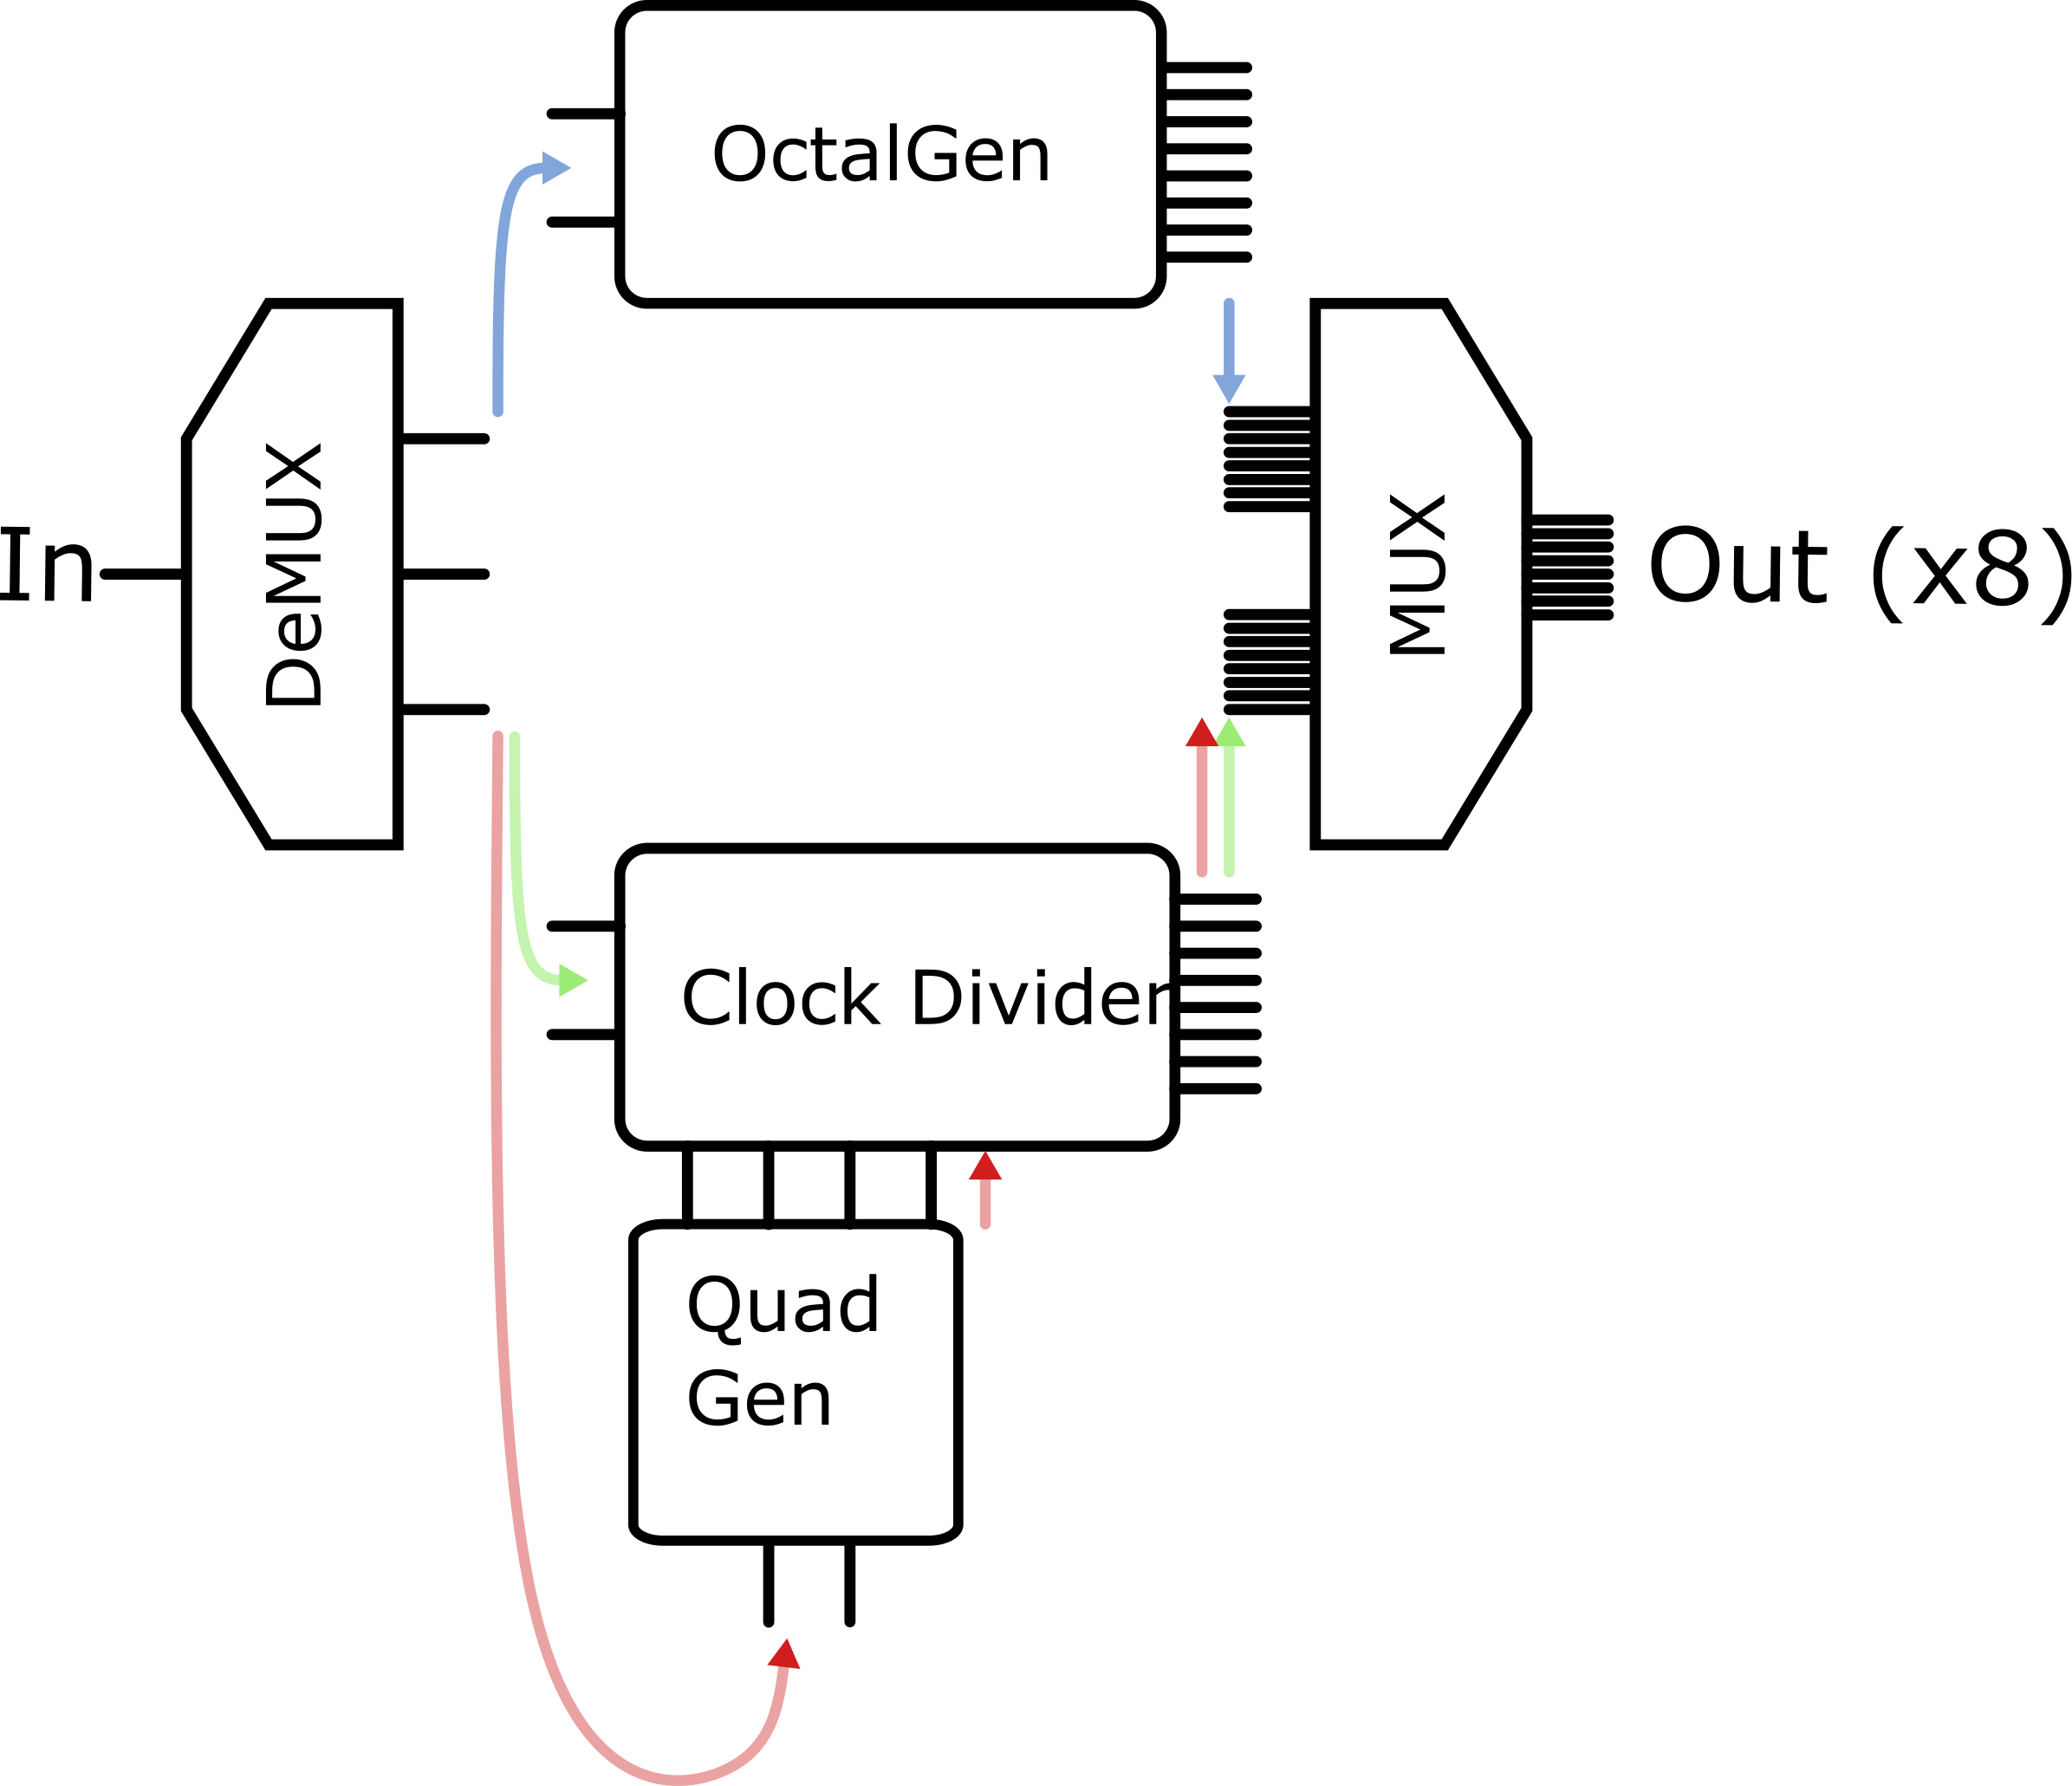
\includegraphics[width=0.5\linewidth]{figures/Schematics/mixF_design.png}
  \caption{Final design architecture with three frequency paths: High-Frequency (HF), Mid-Frequency (MF), and Low-Frequency (LF). The input demultiplexer selects the operational mode, while the output multiplexer combines the outputs from the HF and MF/LF paths.}
  \label{fig:mixF_design}
\end{figure}
An output 2:1 multiplexer selects between the HF and the combined MF/LF output, providing an additional layer of isolation to reduce noise and lower jitter. For design efficiency, the fine-tuning Current-Starved Inverters (CSIs) were placed at the very end of the signal chain, after the output multiplexer. This strategic placement allows a single set of CSIs to correct for skew introduced by all preceding logic, including the input demultiplexer and the main delay stages, regardless of the selected frequency mode.
To further enhance performance, cross-coupling was strategically introduced at critical nodes to improve signal slew rates and guarantee accurate phase spacing.
In subsequent design testbenches, the finetuner was disabled, since the focus was on verifying the functionality of the main delay stages and the ability to produce the clock phases across frequencies and corners with a coarse tuning loop.
\subsection*{Input Demultiplexer and Output Multiplexer Designs}\label{sec:demux_mux_design}
Implementation details and schematics for the input demultiplexer and output multiplexer are provided in Appendix~\ref{app:mux_details}.
\subsection{Octal- and Quad-Generator Designs}\label{sec:octal_quad_gen_design}
The \gls{octalgen} was implemented as the pure delay line design described in Section \ref{sec:second_redesign}, with eight independent delay paths generating the eight output phases. Each path consists of a series of programmable delay elements implemented through capacitive \gls{dac}. The \gls{octalgen} is designed to operate at high frequencies, with the ability to generate clock phases from 11\,GHz to 22.5\,GHz. 
The \gls{quadgen} is used in the MF mode and was implemented as half of the \gls{octalgen}, generating four output phases at the same frequencies and following the exact same design. Importantly, the four output phases are divided once by two using half of the clock divider circuit which will be described below. This frequency division implies the MF path outputs eight phases at half the frequency of the HF path, allowing the design to operate at frequencies down to 5.625\,GHz. Below such frequencies, the LF path is used.
A key consideration in MF mode is the phase spacing between the output clocks. The MF path generates four output clocks that are \ang{90} apart, which are then divided by two to produce eight output clocks that are \ang{45} apart. This implies that tuning phase \ang{90} and \ang{270} is sensed as tuning phase 45 at the output. All other phases are a consequence of the correct spacing between the four output clocks, meaning accurate tuning is achieved by sensing \ang{45} to tune the \ang{90} and \ang{270} phases. This adaptation was implemented as a Verilog-A block that routes the appropriate clock signal to the \ang{90} and \ang{270} CDAC control blocks, ensuring that the correct paths are adjusted for each mode of operation.
\subsection{Low-Frequency Path (Clock Divider) Designs}
The low-frequency path is implemented using a two-stage clock divider composed of flip-flops.
Between the first and second stages, a 2:1 multiplexer selects between the output of the first LF stage and the output of the MF path, allowing the latter to operate at half the frequency of the HF path. This multiplexer is controlled by a simple digital control signal that closes one of two T-Gate switches, connecting either the first stage output or the MF path output to the second stage.
The first stage divides the input clock by two, generating four output clocks at half the input frequency. The second stage further divides these clocks by two, resulting in eight output clocks at a quarter of the input frequency when in LF mode.
In pure LF, there are no addressable skew modulators, since assuming the input clocks are correctly spaced, the output clocks will be perfectly spaced owing to the fully-differential chains and the cross-coupling inverters introduced along the chain. The main design challenges in the LF path were ensuring reliable operation by avoiding metastability and meeting timing requirements across process corners to prevent skipping clock cycles, especially on startup.
\subsubsection{2-stage Divider Design Employing Parallel Flip-Flops}
The schematic of the first implementation for the 2-stage divider is shown in Figure~\ref{fig:2stage_divider}.
This first implementation of the LF path was built for simplicity and robustness, using two identical stages of differential flip-flops arranged in parallel. The first stage consists of two flip-flops, each toggling on the rising edge of one of the input clocks (\(0_{\text{in}}\) and \({180}_{\text{in}}\)). The second stage consists of four identical flip-flops, each sampling one of the output clocks driven by the first stage (\(0_{\text{mid}}\), \(90_{\text{mid}}\), \(180_{\text{mid}}\) and \(270_{\text{mid}}\)). This design ensures that there is enough timing margin for the data input of any flip-flop to settle before the arrival of the next clock rising edge, avoiding metastability and guaranteeing that the output clocks are correctly sequenced. 

\paragraph{Reset Sequence and Logic:}
A critical aspect of the first divider design highlighted above is the reset sequence. Without a proper sequential reset, the flip-flops in the divider circuits can initialize at random states, leading to unpredictable output clock phases, even if relative shifts remain correct. To prevent this, a robust reset sequence was implemented.
The main challenge lay in the fact that, in MF, the reset occurs before the QuadGen is fully tuned, meaning the phase spacing between adjacent clocks (e.g., \ang{0} and \ang{90}) might be too small for cascaded flip-flops to sample correctly. To solve this, the reset sequence is initiated using clocks that are guaranteed to be well-separated. 
In LF mode, the reset is globally triggered by clock \ang{180} from the input, while in MF mode, it is triggered by clock \ang{270} from the quad-generator output. 
Cascaded flip-flops are subsequently arranged in such a way to guarantee that two consecutive flip-flops are clocked by clocks that are at least \ang{180} apart, ensuring settling before sampling. The final arrangement is shown in Figure~\ref{fig:reset_seq}, where the consecutive samplings eventually generate the sequential reset signals after three stages.

\subsubsection{2-Stage "Ring-Oscillator"-like Divider With Clock Slip}
In an attempt to design a reset-free clock divider, a second implementation of the 2-stage clock divider was developed. This design is based on a ring-oscillator-like structure. The schematic of this second implementation is shown in Figure~\ref{fig:div_V2_complete}. 
Setting aside the clock slip and synchronizer, the first stage consists of a single fed-back flip-flop, which samples the input clock and feeds it back to its own data input. The output of this flip-flop is subsequently fed into a set of two flip-flops, clocked at \ang{0} and \ang{180}, leading to the generation of four correctly-spaced output clocks at \ang{0}, \ang{90}, \ang{180} and \ang{270} oscillating at half the input frequency. 
Since the data input of both flip-flops is driven by the same input, the output clocks are guaranteed to be follow the expected \(0\rightarrow 90\rightarrow 180\rightarrow 270\) sequence.
The second clock division stage consists of four cascaded flip-flops, clocked at \ang{180}, \ang{270}, \ang{0} and \ang{90} sequentially along the chain, with the output of the latter stage feeding back into the first stage's data input. This structure guarantees that the output clocks are likewise correctly sequenced.
\paragraph{Clock Slip and Synchronizer:}
Rate-matching between a SerDes transmitter and reciever chain is a common challenge and in some instances perfect frequency alignment is not possible. To address this, a clock slip mechanism is implemented in the clock generator. This mechanism allows the clock divider to slip by one clock cycle, halting data transfer temporarily.
Supposing the transmission chain is running at a slightly higher frequency than the receiver chain, the clock slip mechanism allows the receiver to catch up by skipping a clock cycle. 
In the present design, the clock slip mechanism is implemented using a T-Gate switch connecting the input and output of the feedback inverter in the first stage, while simultaneously disconnecting the inverting common-source inverters from the output (shown in Figure~\ref{fig:div_V2_complete}). This stops the intermediate node in the first stage from toggling, halting the clock generation.

The enable signal for toggling the T-Gate switch must be generated with very good precision such that exactly one period is skipped. This is achieved by using a synchronizer, drawn in Figure~\ref{fig:sync}.
The clock slip enable is asynchronous, simplifying the logic but greatly increasing the risk of metastability. 
To mitigate this, an \texttt{en\_clkslip} signal is generated moments before the clock slip is triggered. This turns on a divide-by-eight chain whose output clocks a set of four cascaded flip-flops. 
The purpose of dividing the clock by eight is to reduce the risk of switching \texttt{pcd\_2UI} (second control signal for the clock slip that actually decides when to slip) too close to a clock edge. This reduces the total number of edges per unit time, which could otherwise lead to metastability due to insufficient timing margin between the data input and clock signal. 

Moreover, the four chained flip-flops have a very high chance of resolving metastability, should it still occur at the first stage. \texttt{pcd\_2UI} must have a total high time of at least eight clock cycles, which guarantees sampling at one edge of the divide-by-eight chain.
This mechanism ensures the \texttt{synced} signal is stable and transitions at a clock rising edge.
As shown in Figure~\ref{fig:div_V2_complete}, the \texttt{synced} signal is the data input of a two-stage flip-flop synchronizer, with the differential outputs of both stages feeding into a fully-differential XOR gate.
After \texttt{synced} rises, the next rising edge of the clock will trigger the first stage of the synchronizer, which will transition the output to high. The second stage will remain low for exactly one clock period, after which it will transition to high. During this intermediate time, exactly one clock cycle, the XOR gate will output a high signal, which is used to enable the T-Gate switch in the first stage of the clock divider, triggering the clock slip mechanism.
\begin{figure}[htbp]
  \centering
  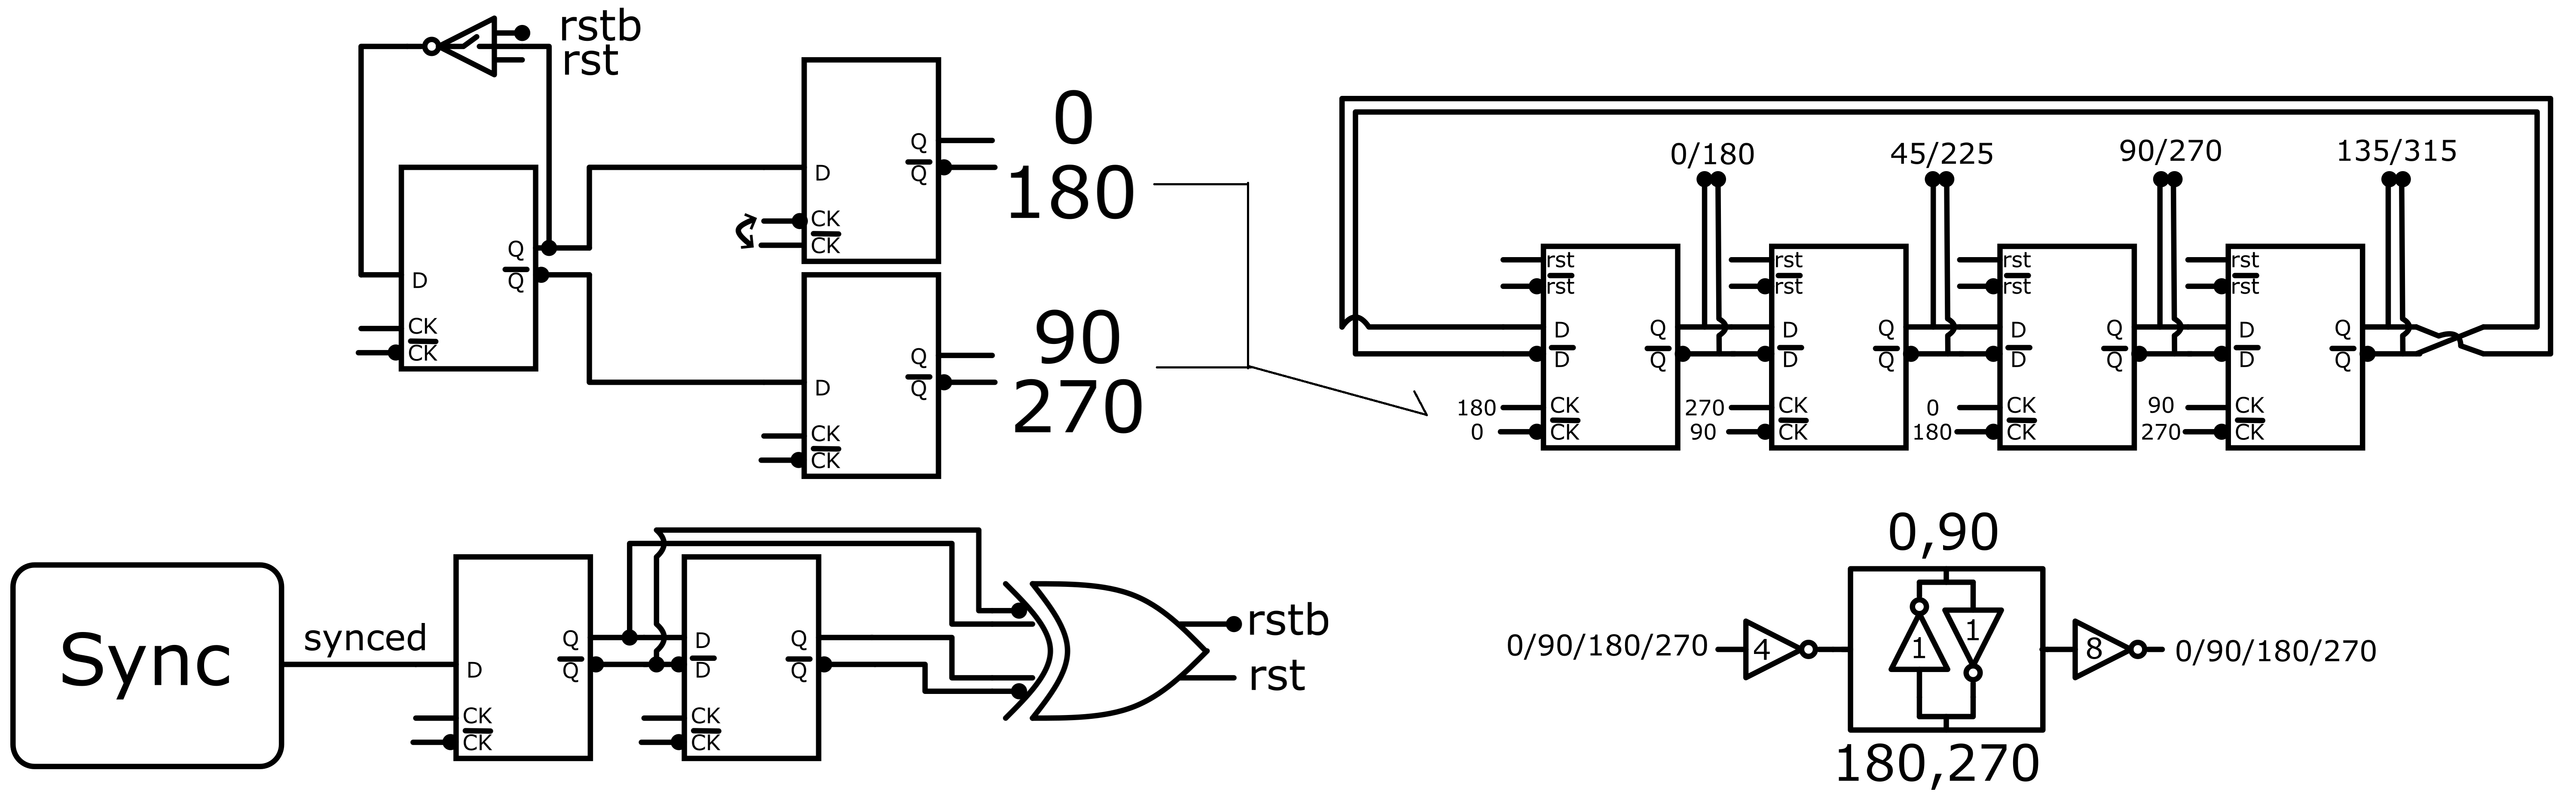
\includegraphics[width=\linewidth]{figures/Schematics/div_V2_complete.png}
  \caption{Schematic of the second implementation of the 2-stage clock divider, based on a ring-oscillator-like structure. The first stage consists of a single fed-back flip-flop, while the second stage consists of four cascaded flip-flops.}
  \label{fig:div_V2_complete}
\end{figure}
\begin{figure}[htbp]
  \centering
  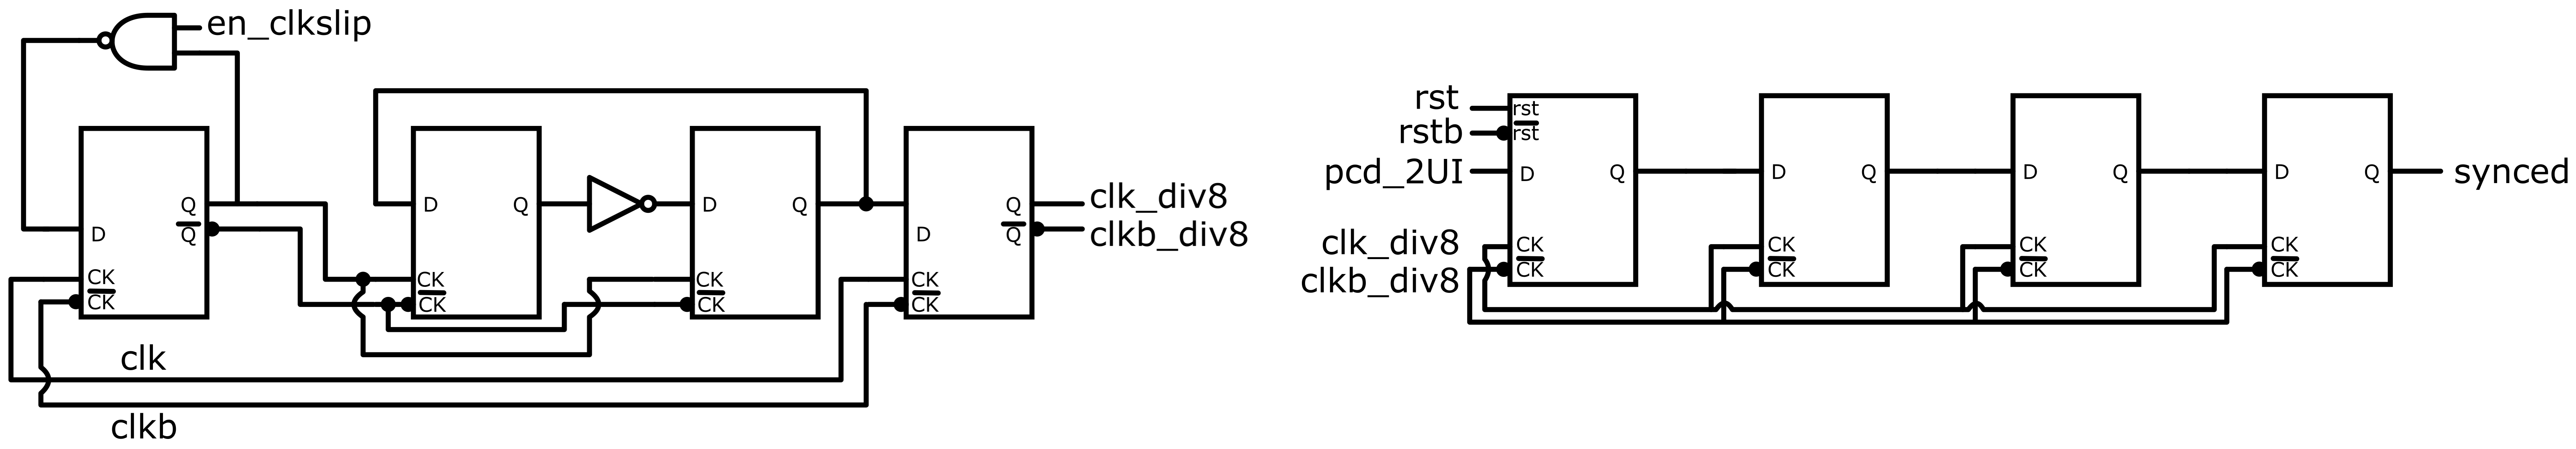
\includegraphics[width=\linewidth]{figures/Schematics/sync_complete.png}
  \caption{Schematic of the clock slip synchronizer. The synchronizer ensures that the clock slip mechanism is triggered with very good precision, allowing exactly one period to be skipped.}
  \label{fig:sync}
\end{figure}
\subsection{Output Fine‑Tuning by Phase Interpolation}\label{sec:output_finetuning}
The final stage of the \gls{mpg} is dedicated to trimming the output clock phases. Capacitance banks were originally intended to remain dynamically programmable so that temperature‑induced drifts could be cancelled in real time. Stress simulations, however, revealed that toggling the \gls{msb} of a bank introduces a transient disturbance: the duty cycle and propagation delay deviate for one, and occasionally two, clock cycles before converging. Although this behaviour did not violate timing in \gls{pvt} corner simulations with the Verilog‑A delay‑compensation wrapper enabled, its magnitude warranted mitigation.
\paragraph{Capacitance‑bank timing study.} Figure~\ref{fig:dcd_MSB} shows the duty‑cycle distortion recorded while forcing an MSB transition at incremental offsets within the clock period. Because each branch carries a phase‑shifted replica of the master clock, simultaneously switching every bank at the ‘optimal’ instant is impossible without per‑branch timing control, additional routing, and removal of the cross‑coupling latches that suppress jitter. Thermometer‑coding the MSBs, which reduces the incremental capacitance step, alleviated the glitch in schematic experiments but increases area and control complexity. We therefore turned to a digital phase interpolator (PI) that can operate continuously while the banks are parked at a safe static code.
\paragraph{Phase‑interpolator architectures.} A tri‑state‑inverter \gls{pi} from an earlier revision provided a convenient starting point: two quadrature input clocks drive parallel tri‑state inverters; enabling/disabling the inverters weights the contribution of each input and hence skews the output phase. Two variants were implemented (Fig.~\ref{fig:phase_interpolators}):
\begin{enumerate}
\item \textbf{Three‑path \gls{pi}} ,  independent tri‑state banks fed by clocks at \ang{0}, \ang{45}, and \ang{90}.
\item \textbf{Two‑path \gls{pi}} ,  one bank driven by the fixed \ang{45} clock; the second is multiplexed between \ang{0} and \ang{90}.
\end{enumerate}
The three‑path topology promises superior linearity but imposes a larger capacitive load on the clock network and demands more control bits. The two‑path topology is both smaller and less intrusive.
\paragraph{Isolation improvement.} Under identical conditions at 22.5\,GHz with seven binary control bits, both \gls{pi} exhibited nearly uniform phase steps. In the two‑path \gls{pi} a single large step appeared during the MUX transition, traced to residual coupling that led to clock feed-through across disabled tri‑state inverters. Relocating the enable switch between the inverter pull devices and the output node improved isolation and removed the glitch. Converting the three \gls{msb} to thermometer code further linearised the transfer and suppressed switching spikes.
\paragraph{Performance summary.} Table~\ref{tab:phase_interpolator_metrics} summarises the simulated results. The two architectures deliver comparable linearity and power, but their \(\approx\)43~fs average step still falls short of the specification. Future iterations will extend the control word by one or two bits to meet the required resolution without compromising jitter.
At this juncture, the \gls{pi} is a credible alternative to the \gls{csi} fine‑tuner discussed in Section~\ref{sec:csi}. The \gls{pi} offers a wide, linear range, whereas the \gls{csi} provides finer resolution over a narrower range. A final decision requires integrating a tuner into the full \gls{mpg} schematic to clarify the required performance trade-offs.
\begin{table}[h]
\centering
\caption{Comparison of key metrics for 2- and 3-path PI finetuning implementations at 22.5~GHz.}
\begin{tabular}{|l|c|c|}
\hline
\textbf{Metric} & \textbf{3-path Implementation} & \textbf{2-path Implementation} \\
\hline
Minimum step (s) & 0 & 0 \\
Maximum step (s) & 68.96f & 71.61f \\
Average step (s) & 42.92f & 43.06f \\
Average power (W) & 4.675m & 4.481m \\
\hline
\end{tabular}
\label{tab:phase_interpolator_metrics}
\end{table}
\begin{figure}[htbp]
  \centering
  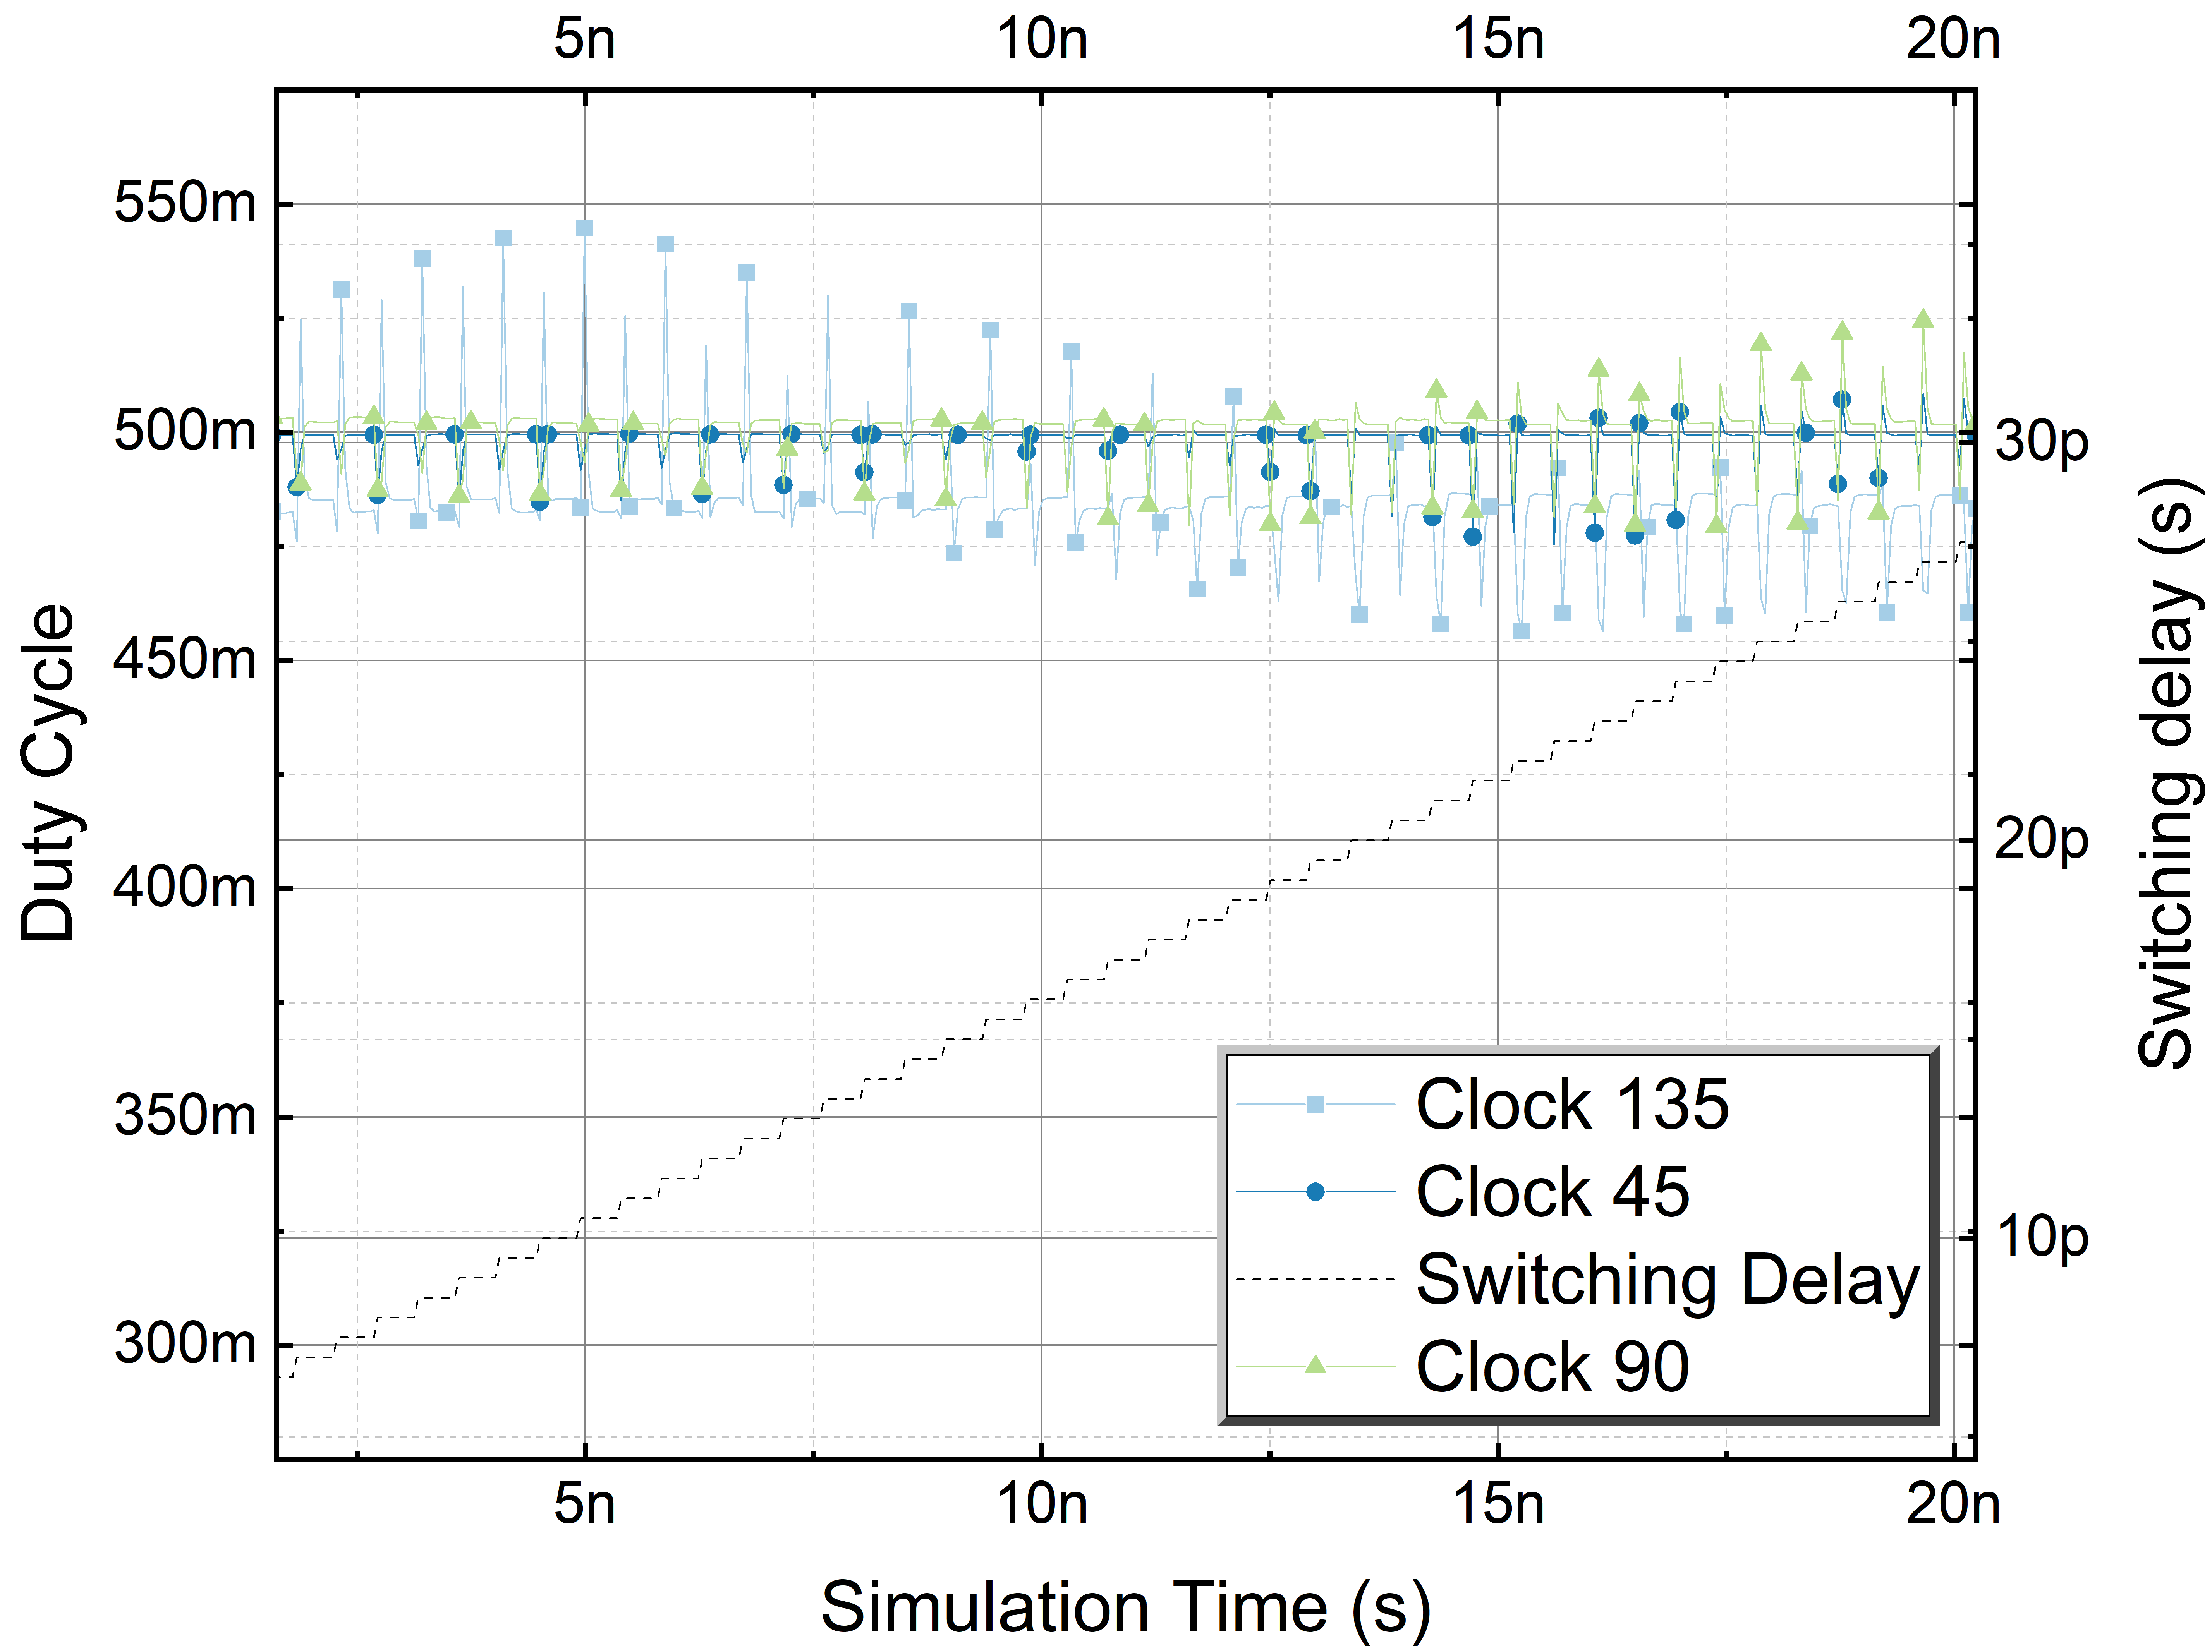
\includegraphics[width=0.4\linewidth]{figures/Results/Final_HF_LF_MF-DCD_vs_switchingDelay.png}
  \caption{duty‑cycle distortion as the MSB switches at different times across the clock period. The duty-cycle distortion is most significant at different times across branches.}
  \label{fig:dcd_MSB}
\end{figure}
\begin{figure}[htbp]
  \centering
  \hfill
  \begin{subfigure}[t]{0.3\linewidth}
    \centering
    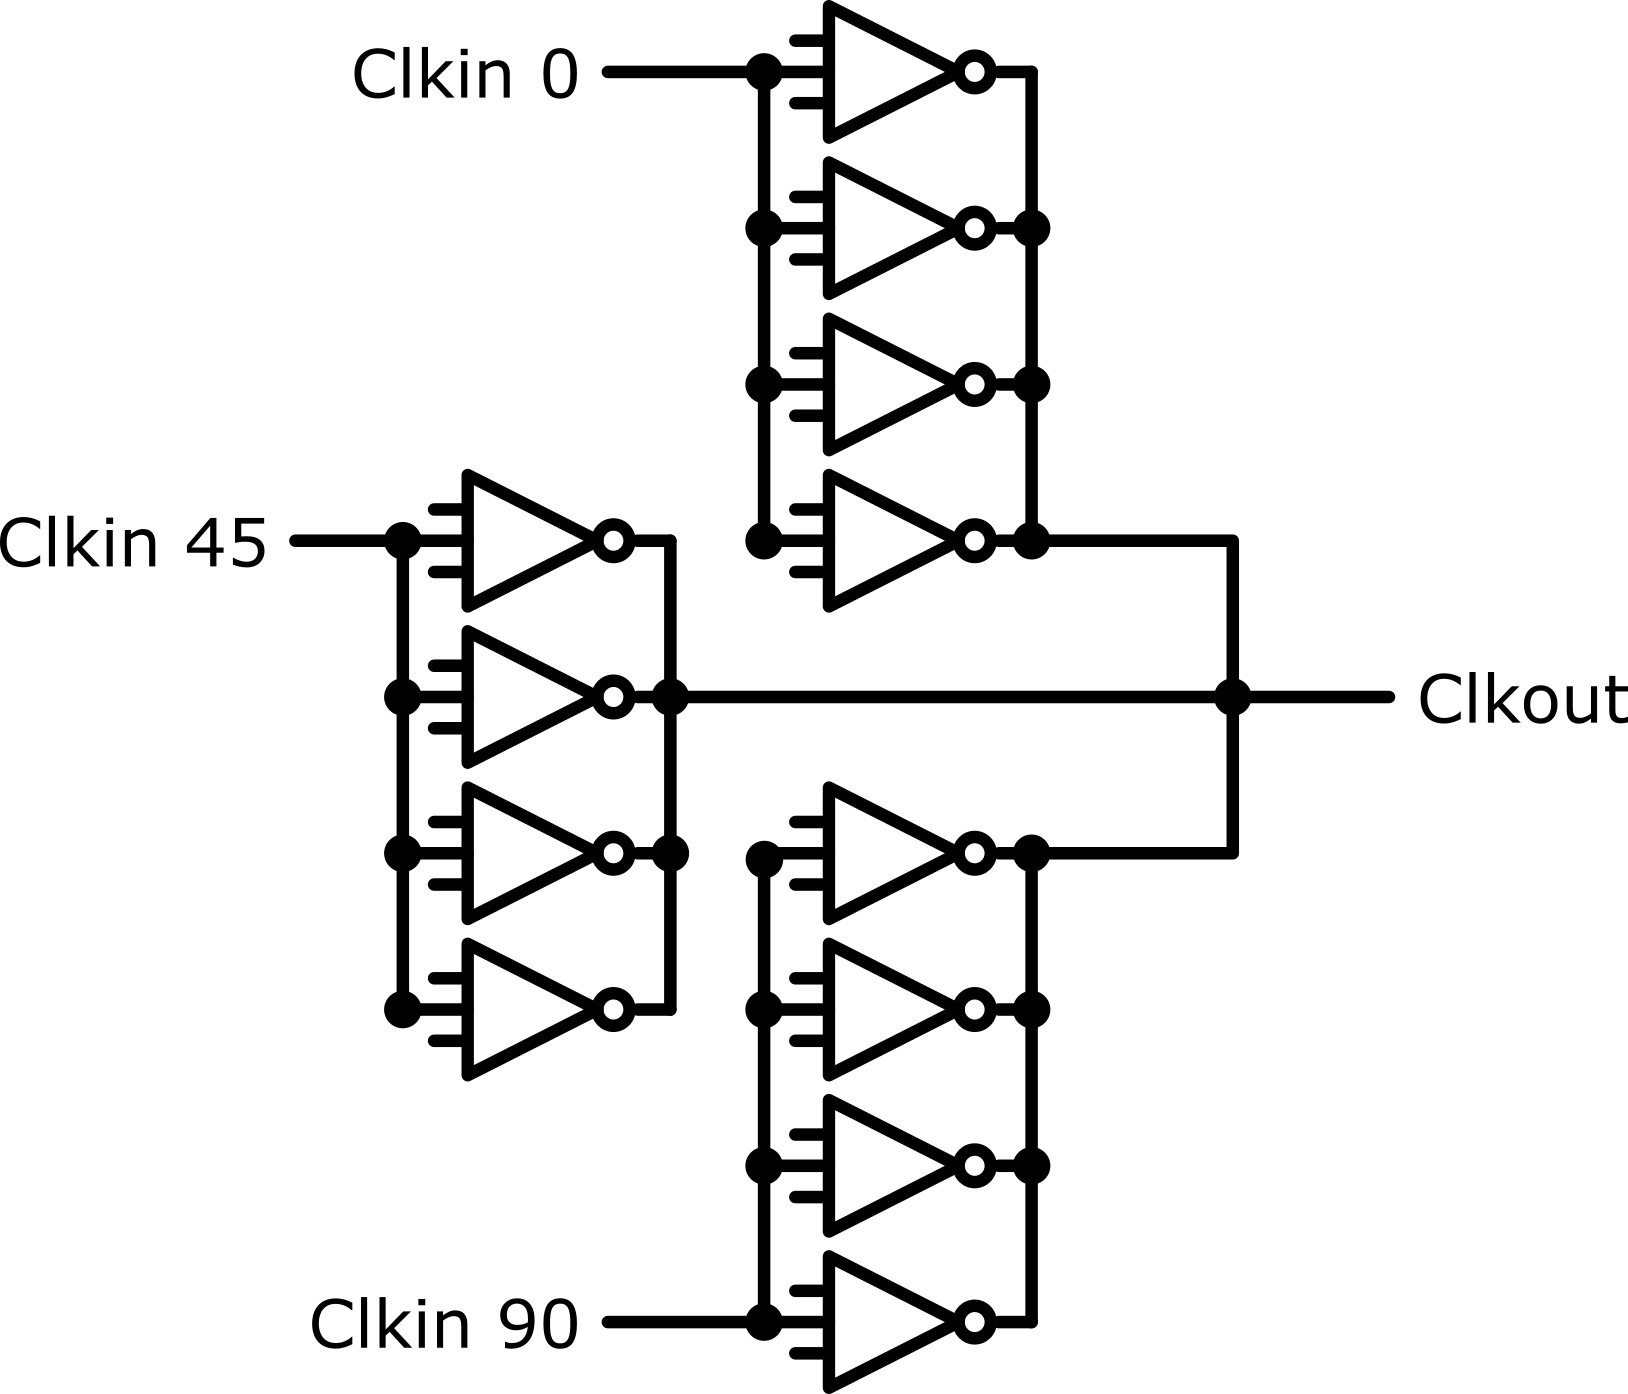
\includegraphics[width=\linewidth]{figures/Schematics/PhaseInterpolator_3paths.png}
    \caption{Phase interpolator with three clock paths (\ang{0}, \ang{90} and \ang{45}) driving tri-state inverters.}
    \label{fig:phase_interpolator_3paths}
  \end{subfigure}%
  \hfill
  \begin{subfigure}[t]{0.3\linewidth}
    \centering
    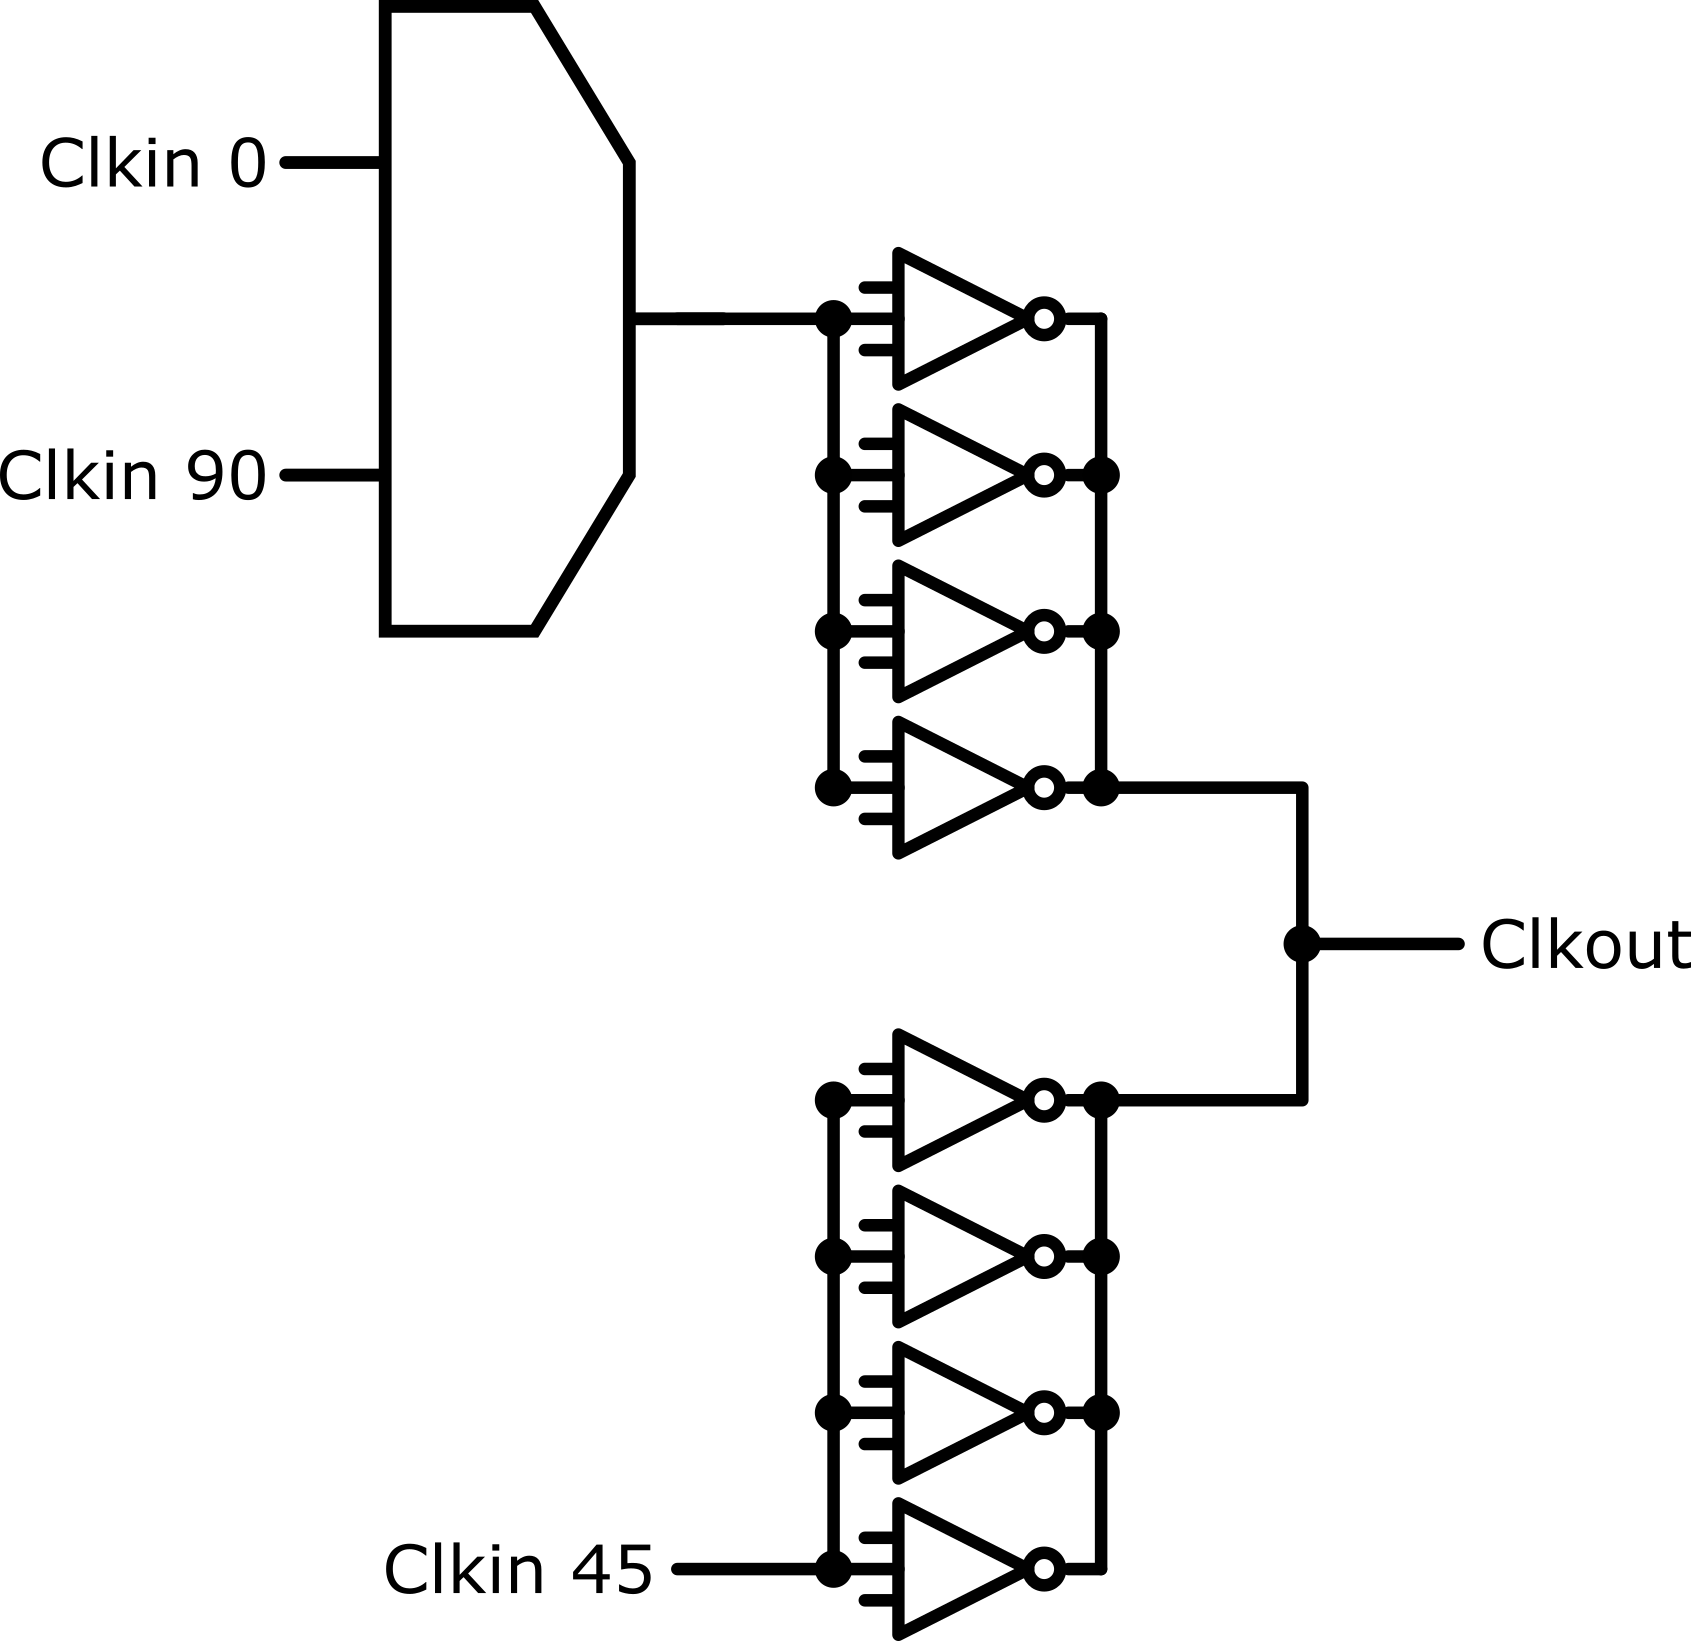
\includegraphics[width=\linewidth]{figures/Schematics/PhaseInterpolator_2paths.png}
    \caption{Phase interpolator with two clock paths (\ang{0} or \ang{90} and \ang{45}) driving tri-state inverters.}
    \label{fig:phase_interpolator_2paths}
  \end{subfigure}
  \hfill\null
  \caption{Digitally-controlled phase interpolators for fine-tuning output clock phases. The first design employs three distinct clock paths, while the second design employs two inverter banks.}
  \label{fig:phase_interpolators}
\end{figure}
\subsection{Key Metrics}\label{final_key_metrics}
The final design of the multiphase generator was evaluated across various process corners and frequencies, achieving promising results. 
Jitter performance was measured at 22.5\,GHz, with the final design achieving an end-to-end jitter below 35~fs (Figure~\ref{fig:final_jitter}). This figure accounts for the jitter introduced by the input demultiplexer, the multiphase generator, the output multiplexer, and two stages of (at this stage, parked) fine-tuning \gls{csi}.
The final capacitor codes were verified to leave an upper and lower margin of around 5 codes over \gls{pvt} (Figure~\ref{fig:final_codes}). This may be insufficient for Monte Carlo drifts, but more range can be easily added by either increasing the number of bits in the capacitance banks or by increasing the step size.
power dissipation was measured with a 22.5\,GHz input, yielding approximately 60~mW in HF mode, 40~mW in MF mode, and 15~mW in LF mode. Figure~\ref{fig:power_consumption} breaks down these figures. As expected, the \gls{octalgen} dominates HF power; the \gls{quadgen} and clock divider contribute roughly equally in MF mode; and the clock divider is the primary consumer in LF mode.
\begin{figure}[ht]
  \centering
  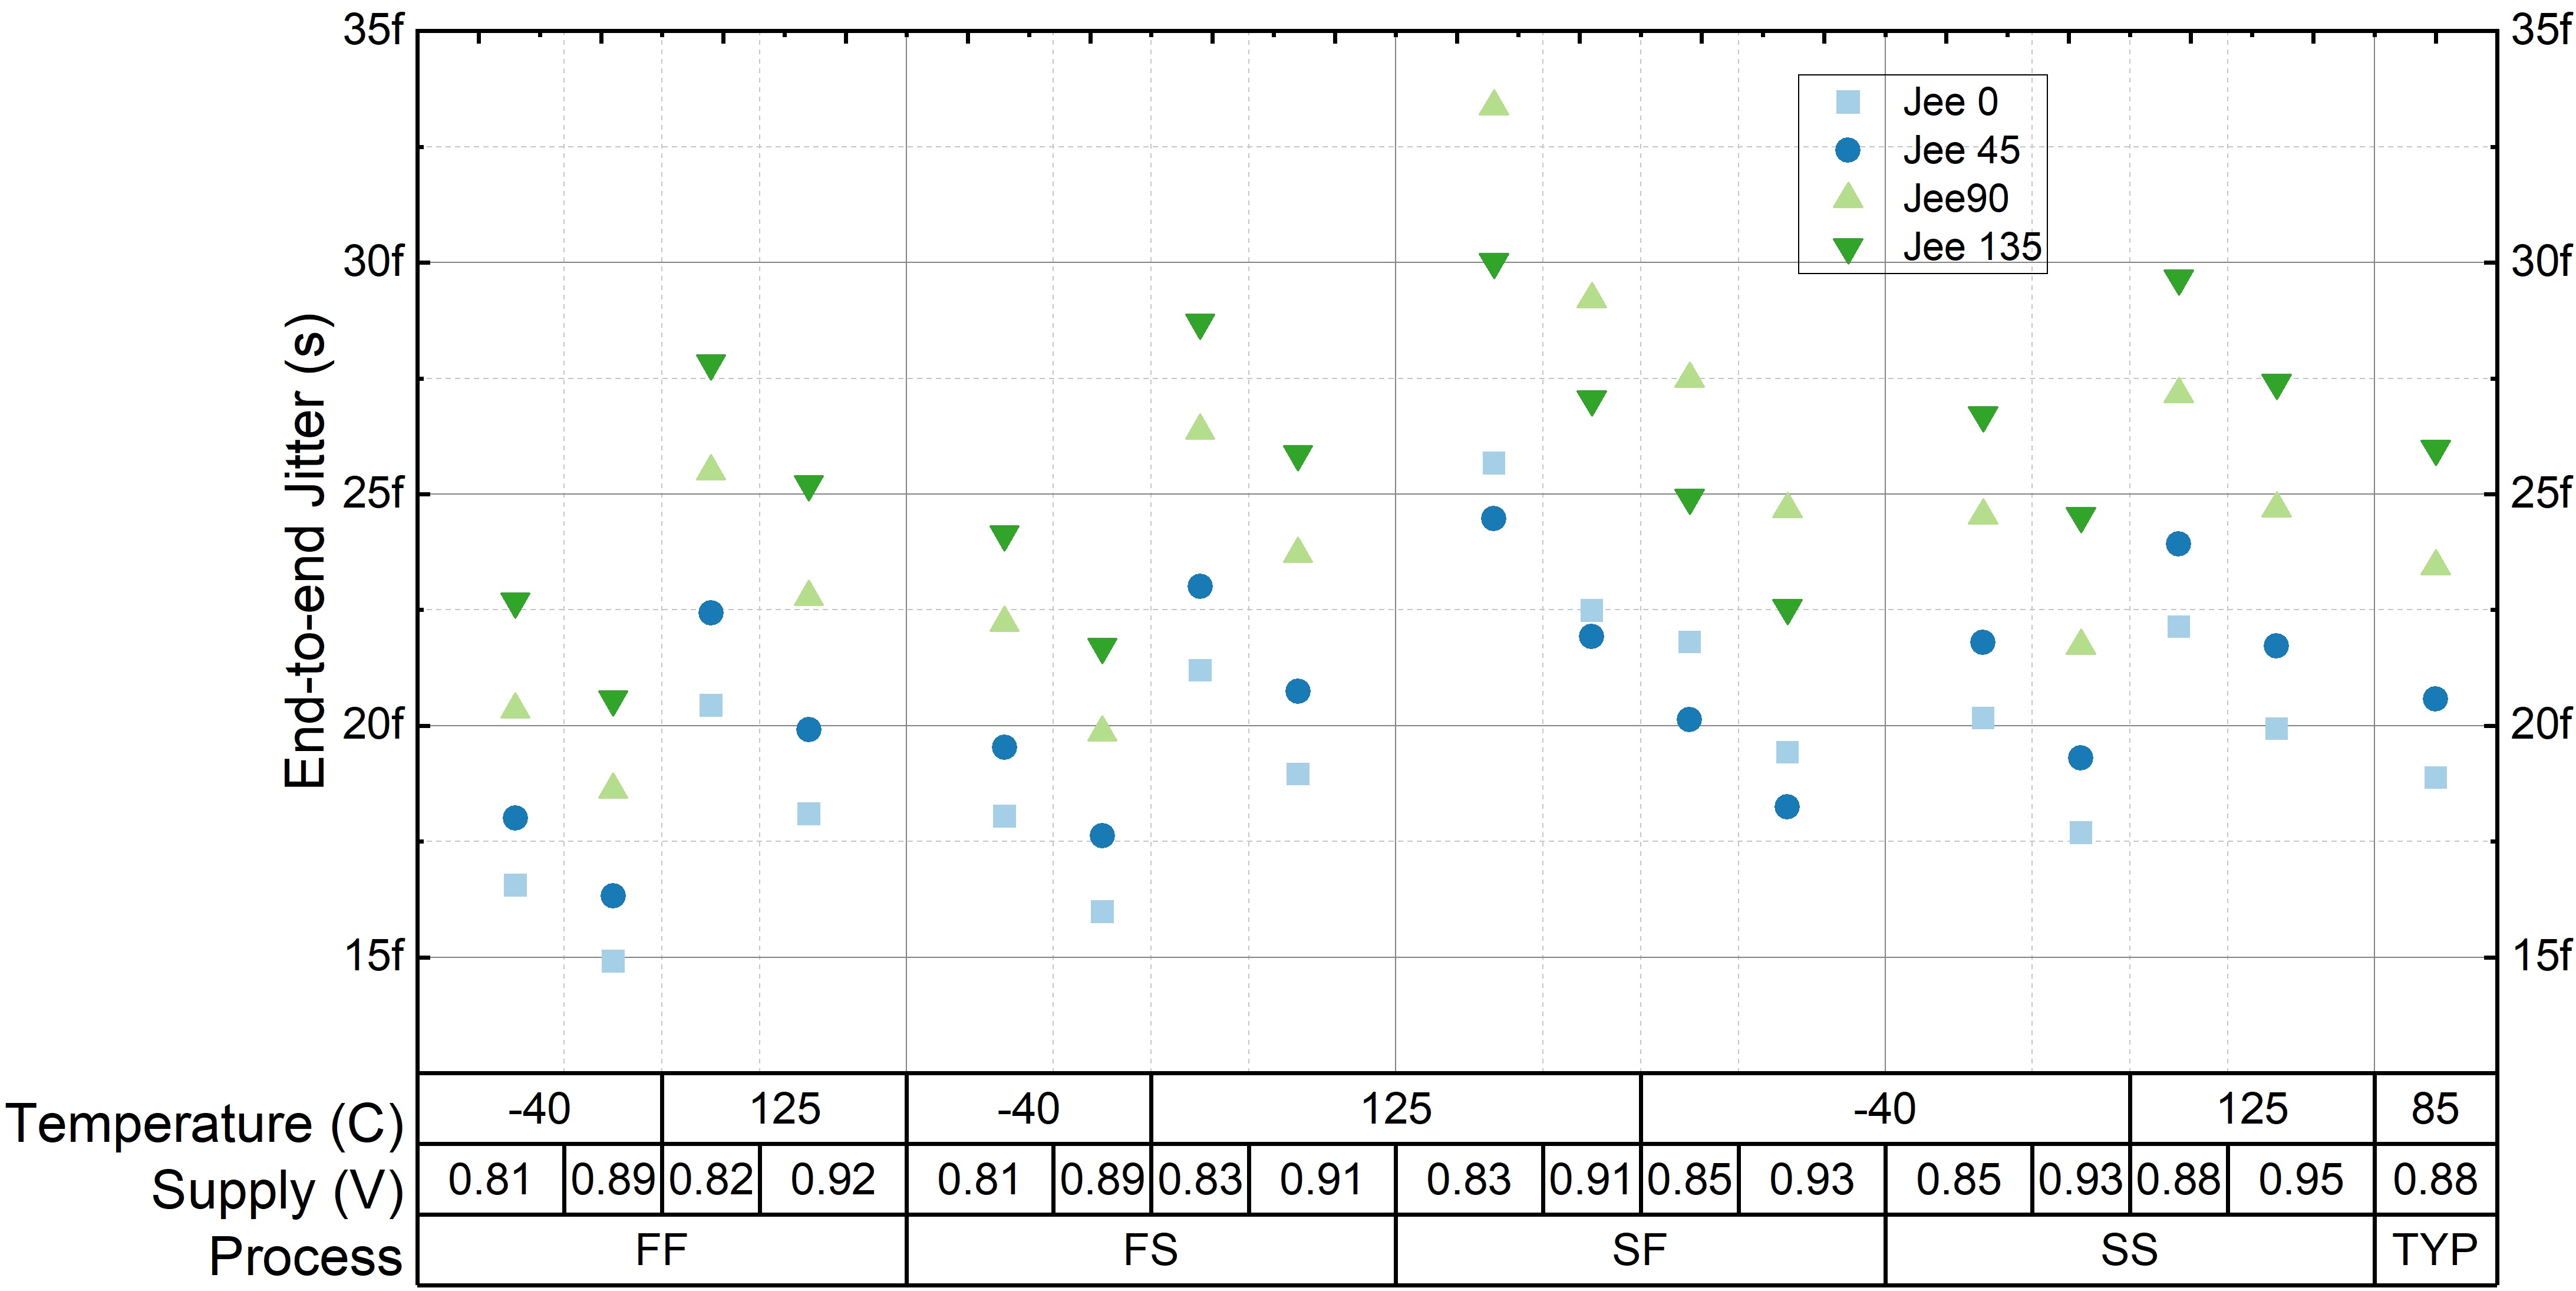
\includegraphics[width=0.8\linewidth]{figures/Results/Final_HF_LF_MF-Pivot_Jee.png}
  \caption{End-to-end jitter performance of the final multiphase generator design at 22.5\,GHz, achieving a jitter below 35 fs across \gls{pvt} corners.}
  \label{fig:final_jitter}
\end{figure}
\begin{figure}[htbp]
  \centering
  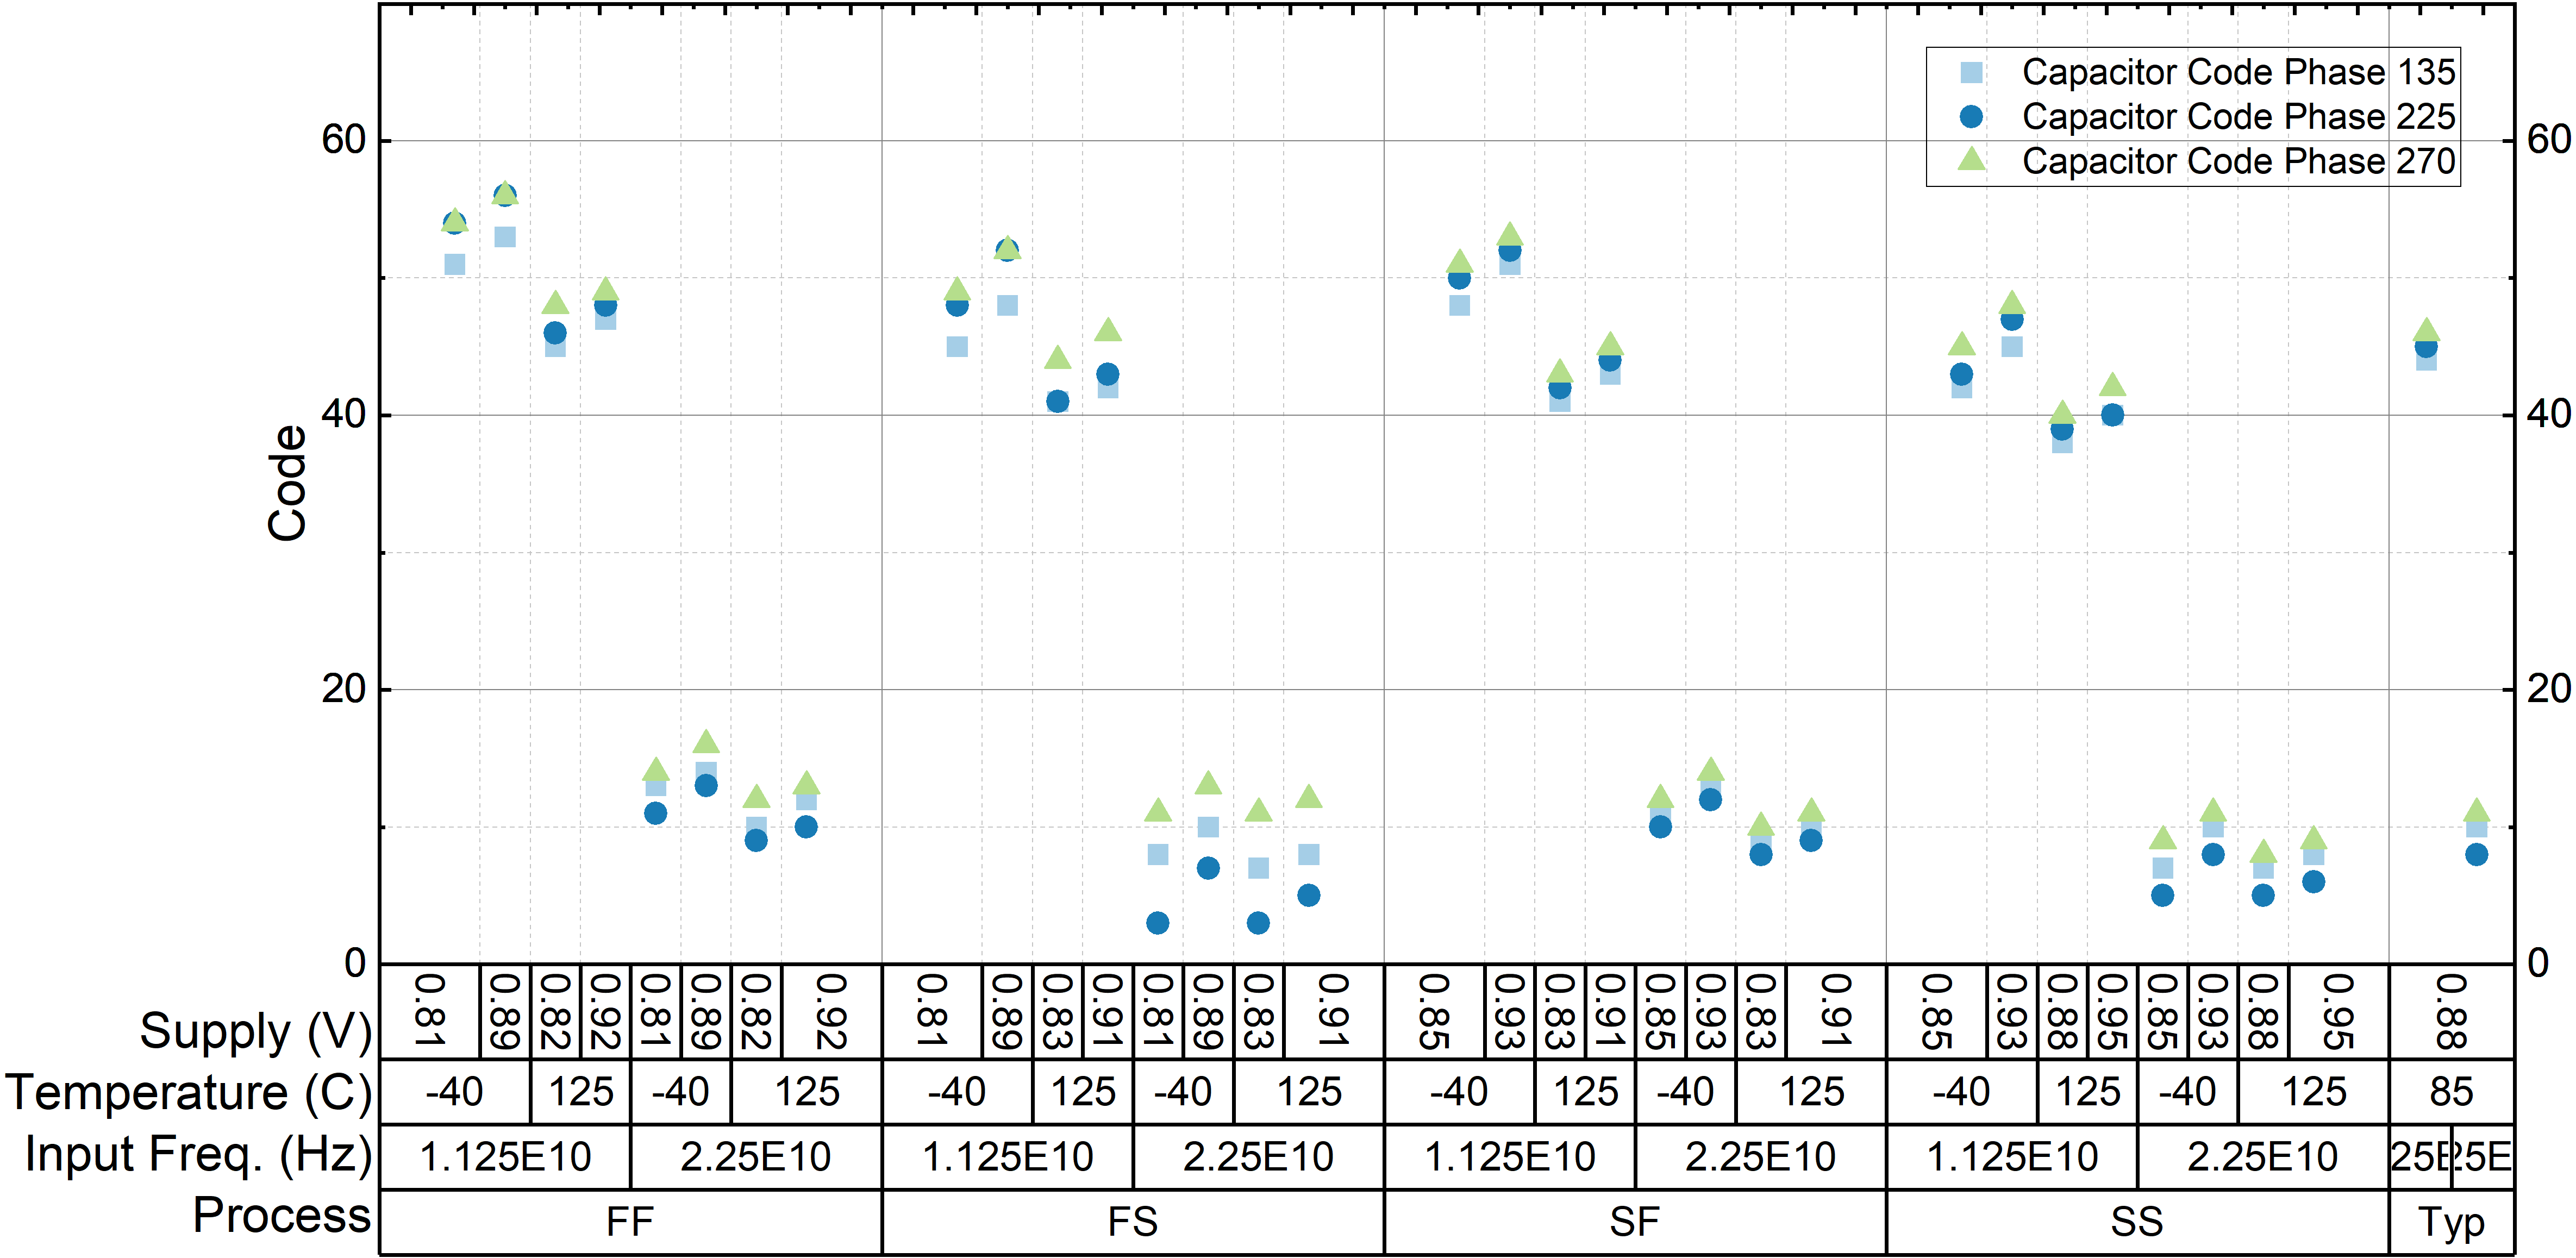
\includegraphics[width=0.8\linewidth]{figures/Results/Final_HF_LF_MF-Pivot_CapCodes_HF.png}
  \caption{Final capacitor codes across \gls{pvt} corners, showing code margins in both directions. The codes are verified to be sufficient for \gls{pvt} correction.}
  \label{fig:final_codes}
\end{figure}
\begin{figure}[ht]
  \centering
  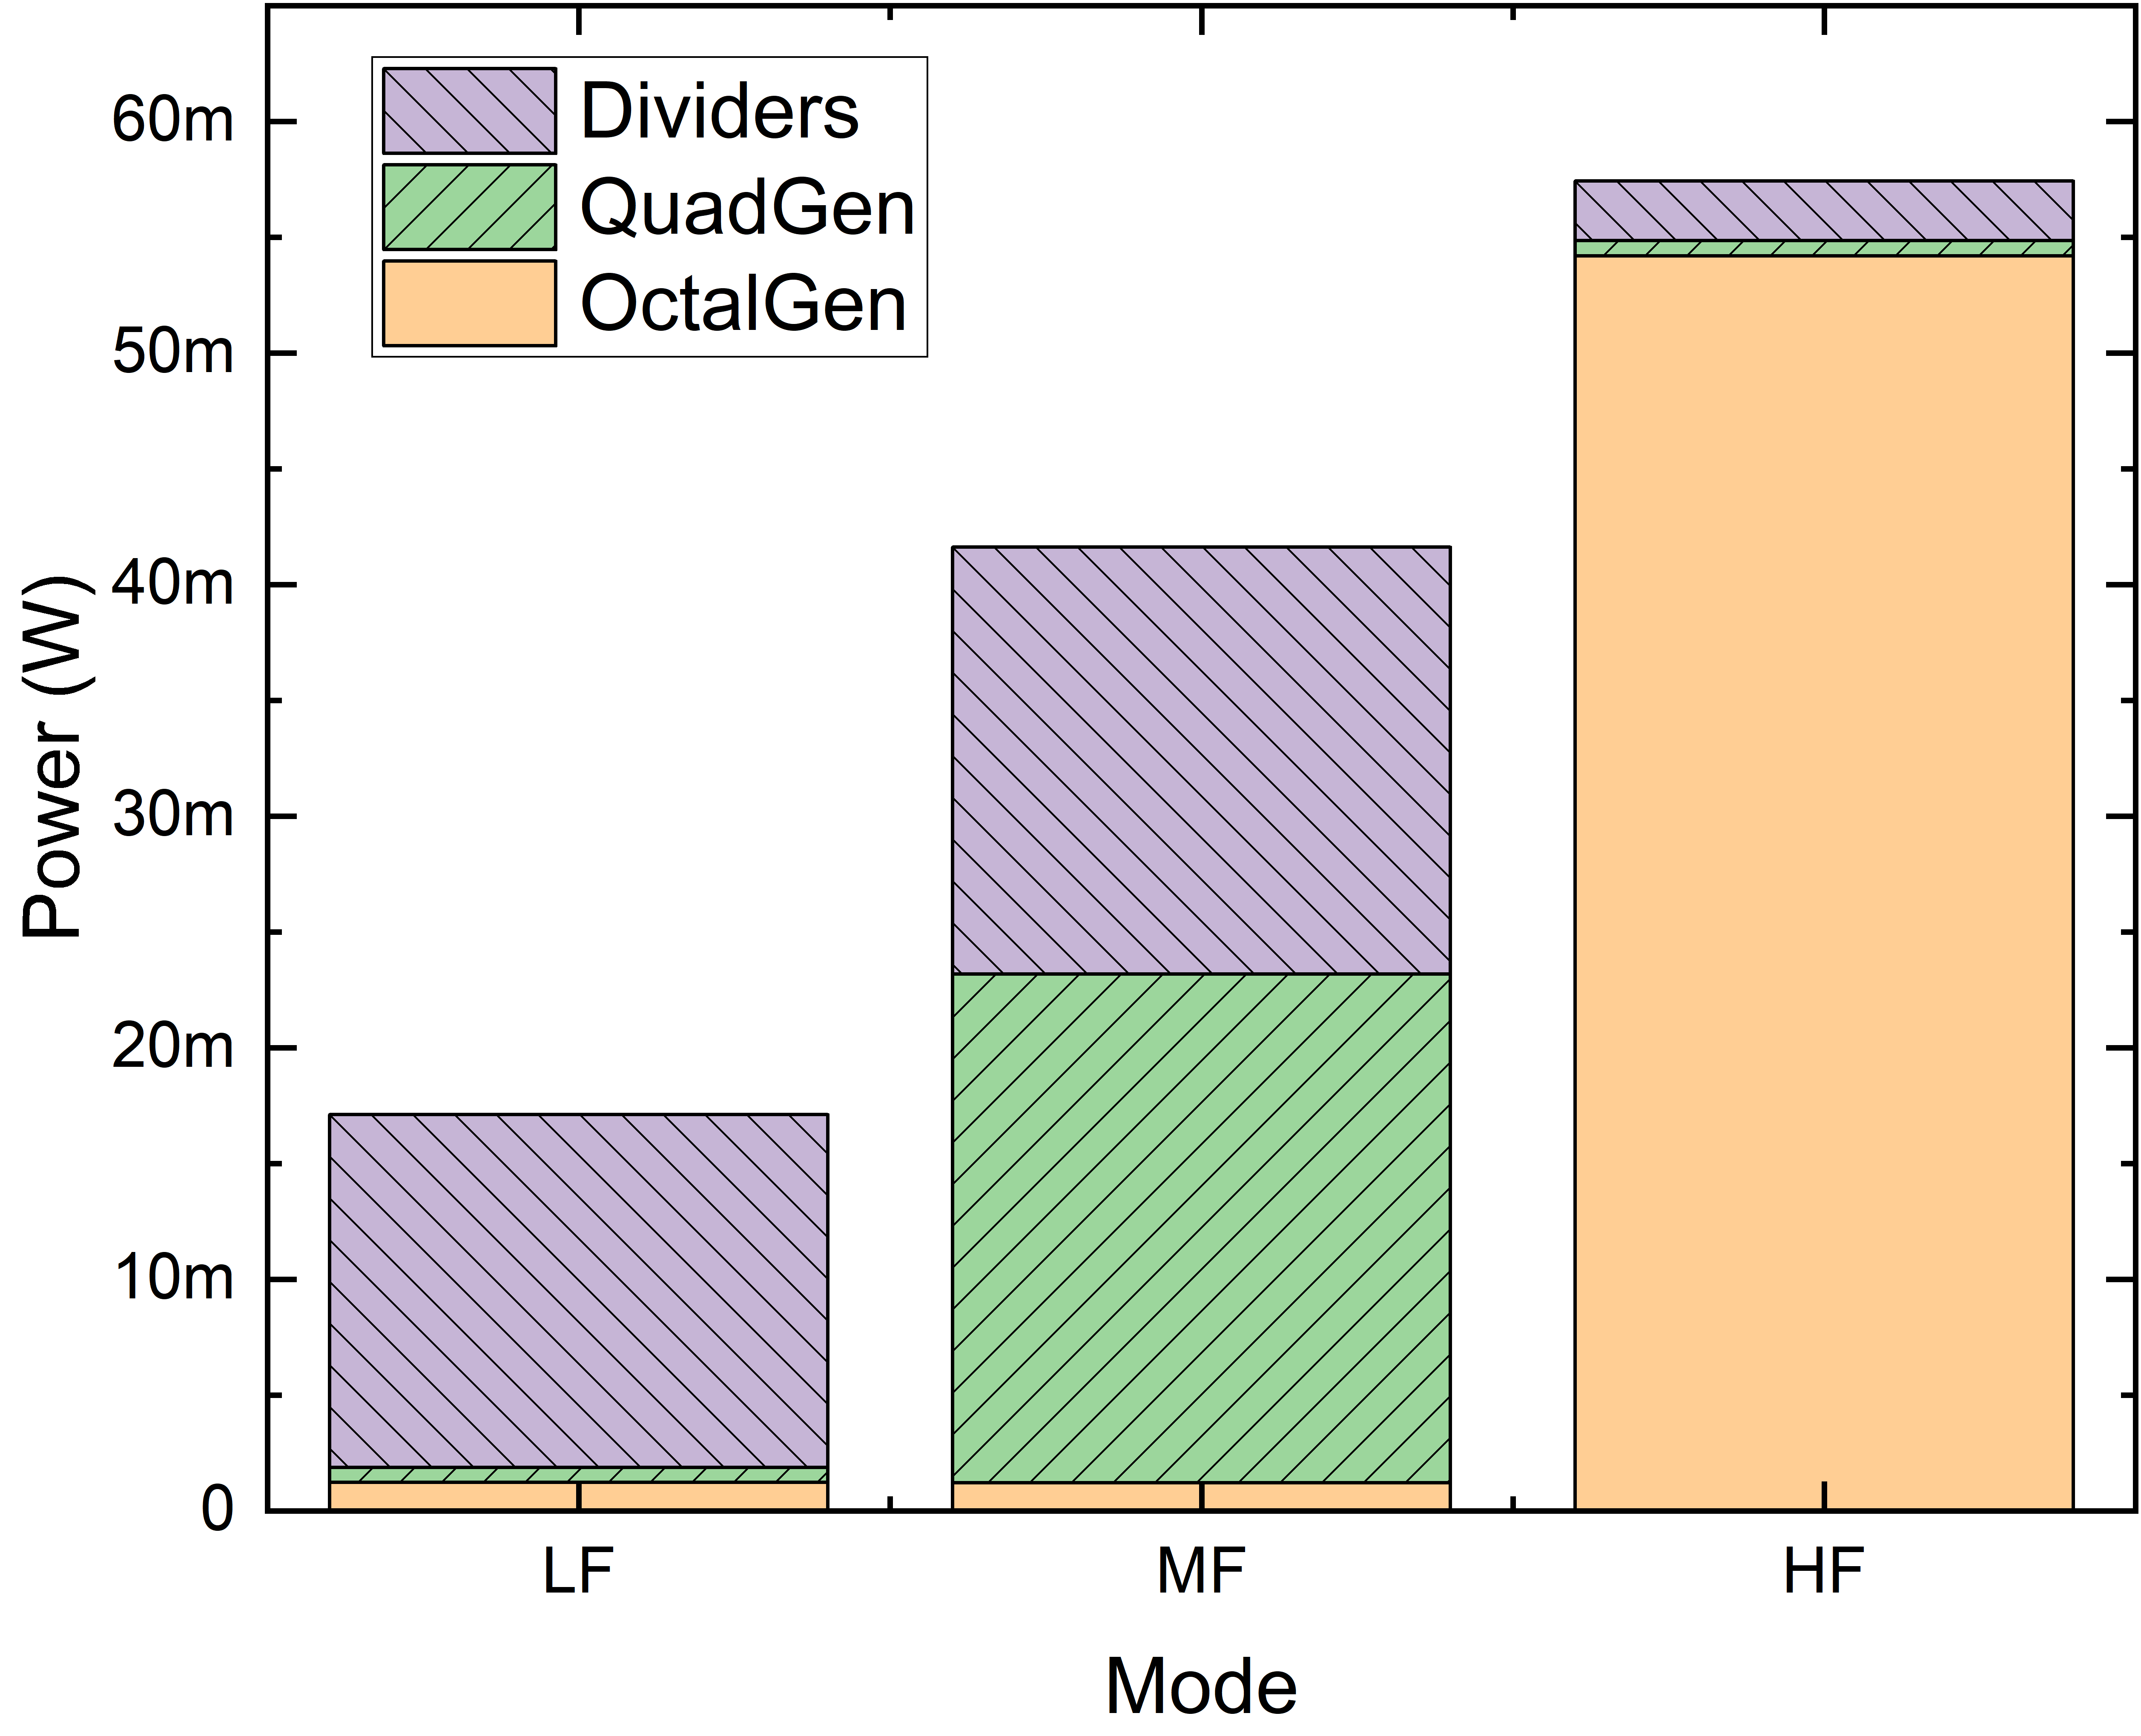
\includegraphics[width=0.4\linewidth]{figures/Results/Final_HF_LF_MF-power_distributions_LFMFHF.png}
  \caption{power dissipation breakdown of the final multiphase generator design across different modes of operation. The charts show the power dissipation contributions of the multiphase \gls{quadgen}, \gls{octalgen} and clock divider, in high-frequency (HF), mid-frequency (MF), and low-frequency (LF) modes.}
  \label{fig:power_consumption}
\end{figure}
Overall, the final multiphase generator design demonstrates robust performance across a wide range of frequencies and process corners, achieving low jitter, efficient power dissipation, and reliable operation in all three modes (HF, MF, LF). The design is well-suited for high-speed clock generation applications in advanced CMOS technologies, providing a versatile solution for generating multiple clock phases with dynamic tuning capabilities.
